% ****** Start of file apssamp.tex ******
%
%   This file is part of the APS files in the REVTeX 4.2 distribution.
%   Version 4.2a of REVTeX, December 2014
%
%   Copyright (c) 2014 The American Physical Society.
%
%   See the REVTeX 4 README file for restrictions and more information.
%
% TeX'ing this file requires that you have AMS-LaTeX 2.0 installed
% as well as the rest of the prerequisites for REVTeX 4.2
%
% See the REVTeX 4 README file
% It also requires running BibTeX. The commands are as follows:
%
%  1)  latex apssamp.tex
%  2)  bibtex apssamp
%  3)  latex apssamp.tex
%  4)  latex apssamp.tex
%
\documentclass[%
 reprint,
%superscriptaddress,
%groupedaddress,
%unsortedaddress,
%runinaddress,
%frontmatterverbose, 
%preprint,
%preprintnumbers,
%nofootinbib,
%nobibnotes,
%bibnotes,
 amsmath,amssymb,
 aps,
%pra,
prb,
%rmp,
%prstab,
%prstper,
%floatfix,
]{revtex4-2}

\usepackage{graphicx}% Include figure files
\usepackage{dcolumn}% Align table columns on decimal point
\usepackage{bm}% bold math
\usepackage{hyperref}% add hypertext capabilities
\hypersetup{colorlinks=true,urlcolor={blue},citecolor={blue}, linkcolor={blue}}
\usepackage{amsmath} % or simply amstext
\newcommand{\angstrom}{\textup{\AA}}
%\usepackage{url}            % simple URL typesetting
%\usepackage[mathlines]{lineno}% Enable numbering of text and display math
%\linenumbers\relax % Commence numbering lines

%\usepackage[showframe,%Uncomment any one of the following lines to test 
%%scale=0.7, marginratio={1:1, 2:3}, ignoreall,% default settings
%%text={7in,10in},centering,
%%margin=1.5in,
%%total={6.5in,8.75in}, top=1.2in, left=0.9in, includefoot,
%%height=10in,a5paper,hmargin={3cm,0.8in},
%]{geometry}

\begin{document}

\preprint{APS/123-QED}

\title{Adatoms in the surface Ullmann couplingk}% Force line breaks with \\
%\thanks{A footnote to the article title}%

\author{Zhenzhe Zhang}
 %\altaffiliation[Also at ]{Physics Department, XYZ University.}%Lines break automatically or can be forced with \\
\author{Dmitrii F. Perepichka}%
 %\email{dmitrii.perepichka@mcgill.ca}
\author{Rustam Z. Khaliullin}
 %\email{rustam.khaliullin@mcgill.ca}
\affiliation{%
 Department of Chemistry, McGill University,\\ 801 Sherbrooke St West, Montreal, QC H3A 0B8, Canada
 %This line break forced with \textbackslash\textbackslash
}%

%\date{\today}% It is always \today, today,
             %  but any date may be explicitly specified

\begin{abstract}
This manuscript reviews the results of experimental and computational studies of the surface Ullmann coupling that shed light on the role of surface adatoms in its mechanism. A particular focus is on the early stages of the polymerization and coupling of two monomers.
%\begin{description}
%\item[Usage]
%Secondary publications and information retrieval purposes.
%\item[Structure]
%You may use the \texttt{description} environment to structure %your abstract;
%use the optional argument of the \verb+\item+ command to give the category of each item. 
%\end{description}
\end{abstract}

%\keywords{Suggested keywords}%Use showkeys class option if keyword
                              %display desired
\maketitle

%\tableofcontents

\section{\label{sec:level1}Introduction\protect\\ %The line
%break was forced \lowercase{via} \textbackslash\textbackslash
}

\subsection{\label{sec:level2}Ullmann coupling in solution}

%ZZ:(Cu is called ac active species in the whole manuscript, cause I found it is oxidized)
%ZZ:(only refer to C-C bond)
Cu-containing arylation which mainly referred to the formation of C--C and C--X(X = O, S and P) bonds has acquired great importance in the last decades. This type of reactions could trace back to one of the oldest reactions, named Ullmann reactions.
In 1901, Fritz Ullmann discovered~\cite{ullmann_01} a coupling reaction that results in the construction of a C--C bond between two aryl halides in the presence of an equivalent amount of Cu powder.
%RZK is the previous statement correct? or should we use the alternative ending below?: in the presence of Cu-containing catalysts. (%ZZ: in Ullmann's disvocery, he used Cu powder)

Today, terms ''classical'' Ullmann, Ullmann-type or simply Ullmann reaction refers to a family of Cu-containing compounds utilized to initialize nucleophilic aromatic substitution between various nucleophiles with aryl halides.
%(RZK: aromatic?) %(ZZ: solved) 
%RZZK-original: The ''classical'' Ullmann reaction, named after Fritz Ullmann who discovered it in 1901~\cite{ullmann_01}, is a coupling reaction between two aryl halides that results in the creation of a C--C bond between the aromatic rings in the presence of Cu-containing catalysts (figure.~\ref{fig:classical}).
With increasing understanding of the mechanism towards transition-metal mediated reactions, the scope of the Ullmann coupling reaction has been extended to new reactants and active species, to construct other covalent bonds like C--N~\cite{ullmann_02, ullmann_03}, C--O~\cite{ullmann_04}, C--S~\cite{ullmann_05} and C--P~\cite{ullmann_21,ullmann_22} bonds, as shown in Fig.~\ref{fig:UllmannCoupling}\cite{ullmann_30}.
\begin{figure}[htb]
\centering
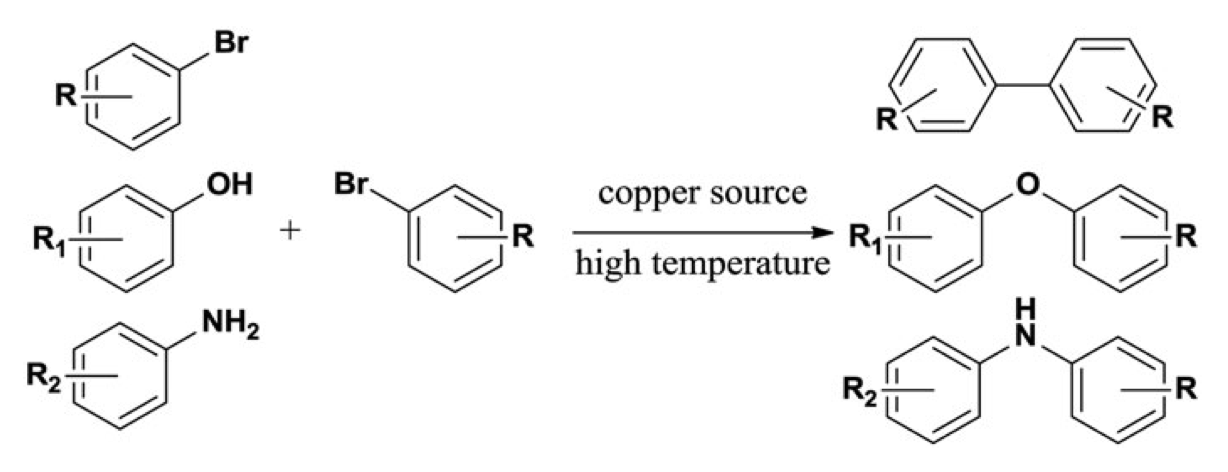
\includegraphics[width=0.75\columnwidth]{Fig/classical.png}% Here is how to import EPS art
%RZZK: "Cu source" -> "Cu source"; "high T" -> "high T"(ZZ: could I use the full sentence: high temperature?)
\caption{Examples of Ullmann coupling reaction which could construct C--C, C--O and C--N bonds.}
\label{fig:UllmannCoupling}
\end{figure}
%RZK: diary ether??? phosphines and/or phosphites? (%ZZ: solved, typo)

Depending on the type of bonds created, reactants in the Ullmann coupling reaction include aromatic amines~\cite{ullmann_17,ullmann_18} and amides~\cite{ullmann_19,ullmann_20} for the C--N bond creation; phosphines~\cite{ullmann_21,ullmann_22} to achieve the arylation of phosphines; carboxylic acids~\cite{ullmann_23}, diaryl ether~\cite{ullmann_24}, phenols~\cite{ullmann_25} and other oxygen-containing species~\cite{ullmann_26,ullmann_27,ullmann_28} to obtain C--O bond products.

Halogens as leaving groups are most common in the substitutions. While iodine and bromine serve as very popular leaving groups in Ullmann coupling, tosylate as leaving group has also been reported~\cite{ullmann_15}. 

As for the active metal species, Cu-containing compounds are most widely used among all type of metals. In addition to Cu(0), different Cu(I) and Cu(II) salts and oxides -- including CuI~\cite{ullmann_07,ullmann_08,ullmann_09}, $CuBr$~\cite{ullmann_10,ullmann_11}, $CuCl$~\cite{ullmann_13}, $Cu_2O$~\cite{ullmann_12}, $Cu(acca)_2$~\cite{ullmann_14}, $Cu(OTf)_2$~\cite{ullmann_15}, $CuO$~\cite{ullmann_16} -- have also been used. Apart from Cu-containing compounds, Pd–Fe~\cite{ullmann_35} and Au–Pd~\cite{ullmann_36} Nanocomplexes have also been proven be effective in Ullmann coupling reaction. The Ullmann coupling reactions discussed above occur mostly in organic solvents. 

Currently, the scope of Ullmann coupling reaction is being widened with an increasing number of substrates, leaving groups, and active metal species being investigated for constructing various C--X bonds. 

% RZZK: other metals as catalysts? Yes. But is it called Ullmann in this case? (%ZZ: yeah, I listed all the metal compounds used)

%RZZK, our next major task is to describe the mechanism using the commonly accepted terminology. (%ZZ: Cu(I) actually is the catalyst species)
The mechanism of Ullmann coupling reaction in solution is also well developed. It is universally accepted that the Ullmann coupling proceeds via the formation of an organometallic intermediate. Taking the Ullmann coupling of bromobenzene with Cu for instance, the bromobenzene molecule firstly approaches the copper species to form an aryl organometallic intermediate. Then this intermediate would react with another precursor to form a diaryl organometallic intermediate. Followed by a reductive elimination, the product biaryl moiety is obtained, the general mechanism is shown in Fig.~\ref{fig:classical}.~\cite{ullmann_37}.

\begin{figure}[htb]
\centering
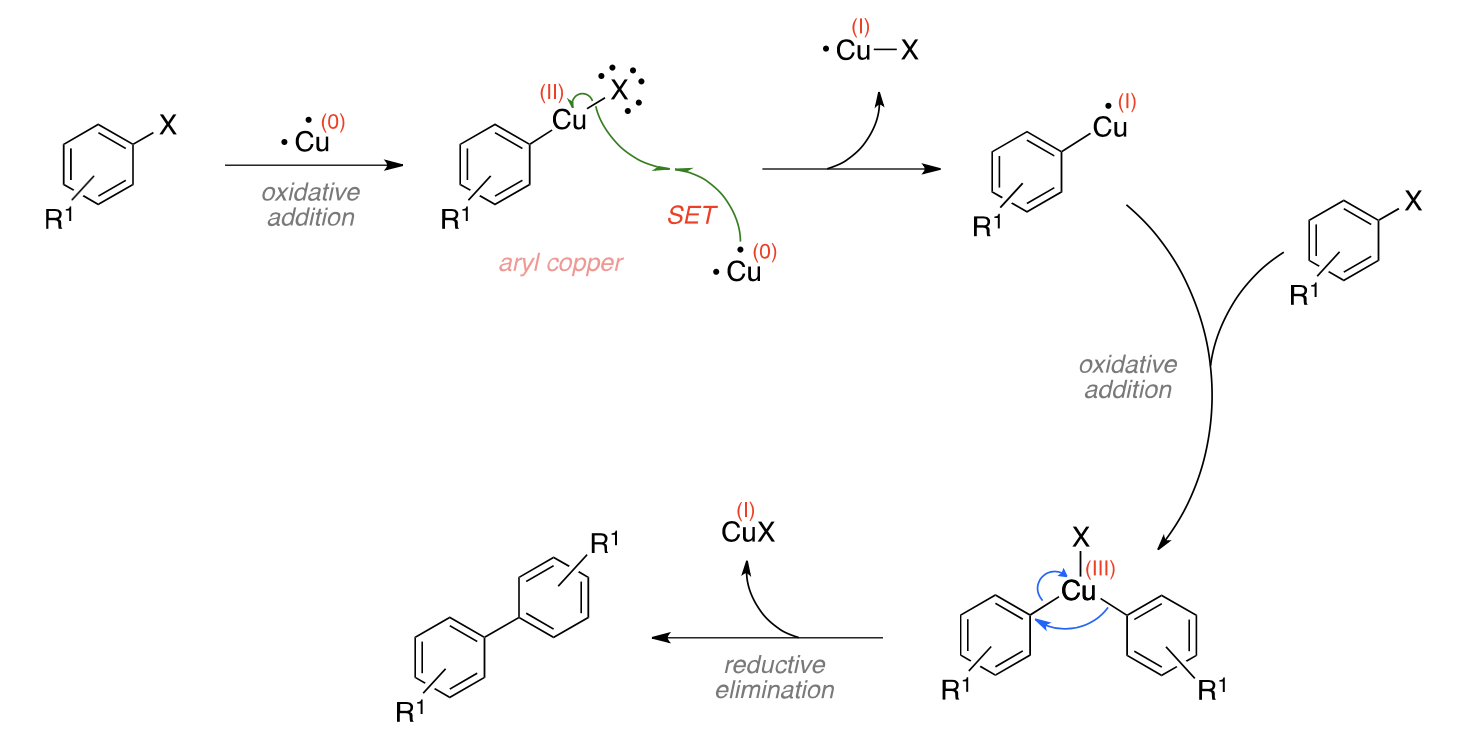
\includegraphics[width=0.90\columnwidth]{Fig/classical-mechanism.png}
% RZZK: This looks like a very clear figure that explains the mechanism. Some modifications will be necessary LATER: 
% * convert into a one-line page-wide scheme. (%ZZ: done)
% * clarify whether Cu is a reactant or catalyst. If latter, it is unclear how Cu returns to its initial Cu(0) form. (%ZZ:I call it active species, then this issue solved)
% * why Cu(0) is shown with two electrons? Is it better to show Cu without its electrons?
% * define SET: single-electron transfer? (%ZZ: add in figure caption)
% * How is it possible to use Cu(II) salts as catalysts/reagents? 
\caption{General mechanism of the Ullmann coupling reaction with Cu active species, $Cu[I]$ is the actual catalyst in the reaction. (SET: single-electron transfer; the black dots are referred to the electrons around Cu which could distinguish $Cu[0]$, $Cu[I]$, $Cu[II]$)}
\label{fig:classical}
\end{figure}
Cu-containing Ullmann coupling has acquired great significance in the last decade due to its advantages such as (1) Cu is a cheaper alternative to palladium, platinum or rhodium,  (2) avoidance of the halogen side-products; and (3) air or oxygen can act as oxidants~\cite{ullmann_38,ullmann_39,ullmann_40,ullmann_41}. However, drawbacks still exit for large-scale development: (1) harsh conditions are necessary like high temperature and polar solvents with high boiling point; (2) poor solubility of many Cu compounds in organic solvent; (3) poor functional groups tolerance~\cite{ullmann_31}. Despite a variety of limitations mentioned above, the Ullmann coupling has become and still remains one of the key reactions to build C-C bonds in organic synthesis. 

Recent advances of Ullmann coupling reaction in solution have been reviewed by several authors~\cite{ullmann_29,ullmann_30,ullmann_31,ullmann_32}.

%RZK: Reaction mechanism figure for Cu(I) or Cu(II). Catalyst regeneration.
%ZZ: actually there is in investigation that Cu(I) is the real catalyst in Ullmann coupling reaction~\cite{ullmann_31}, we should discuss in details or just use active species?)

\subsection{Surface Ullmann coupling}

A recent surge of interest in electronic devices based on low-dimensional organic nanostructures with $\pi$-conjugated backbones has led to a renewed attention to the Ullmann coupling reaction. 
In the case of low-dimensional materials, the well-established ability of the Ullmann coupling to create bonds between aromatic carbon atoms and couple their $\pi$ systems have been transferred from solution to metal surfaces, which serve as both a low-dimensional confining template and catalyst.

The on-surface Ullmann reaction is currently viewed as a promising bottom-up strategy to assemble, in mild conditions, one- and two-dimensional organic polymers with high degree control of their electronic properties~\cite{ullmann_33}. 
In the context of surface reactions, the term Ullmann coupling has been extended to refer to the reaction on metals other than Cu, such as silver and gold. 

% RZZK. They say, phenyl is parallel to the surface. Was it confirmed later? (%ZZ: not understand)
One of the first fundamental studies of the surface-confined coupling of iodobenzene to biphenyl under ultrahigh vacuum (UHV) condition was reported by Xi and Bent~\cite{sur_sci01} in 1992.
The intermediate phenyl group of this reaction were inspected using STM imaging by Weiss \textit{et al.}~\cite{langm01} in 1998.
% RZZK: I removed the following reference because it cannot be classified as Ullmann coupling
% STM tip was further utilized to achieve a chain polymerization, which result in polydiacetylene from diacetylene compounds in 2000~\cite{ullmann_34}.
In 2004, it was demonstrated that linear \emph{protopolymers} (aligned monomer units of a polymer that have not yet reacted to form the final polymer) could be obtained by depositing \textit{para}-diiodobenzene on Cu(111) at 77 K~\cite{jacs01}. This breakthrough provided a new insight that not only could simple organic molecule be synthesized by surface Ullmann coupling, but periodic polymer as well.
Remarkably, the first synthesis of covalently-bonded nanostructures from molecular building blocks on metal surfaces under UHV has employed surface Ullmann reaction: the coupling between brominated tetraphenyl-porphyrins on the Au(111) surface was performed by Grill \textit{et al.}~\cite{Naturenano2007} in 2007.

Since then, surface Ullmann coupling has become one of the most representative on-surface synthesis scheme and has been utilized to create a variety of covalently-linked extended aromatic systems from halogenated aryl precursors on multiple metal surfaces~\cite{ullmann_33,ullmann_34, ullmann_42, ullmann_43, ullmann_45, ullmann_46, ullmann_47, ullmann_48}. 
%RZK: more reviews from our list must be cited here (%ZZ: done)

\subsection{Mechanism of surface Ullmann coupling}

Although multiple covalently-bonded nanostructures have been obtained on metal surfaces via Ullmann coupling, our knowledge of the mechanism of the surface processes still remains fragmentary. 
%
A thorough understanding of the mechanism of surface Ullmann coupling reaction will enable rational, faster, more precise design of the halogenated precursors, well-matched to a chosen metal surface.
%
%RZZK: the following sentence does not belong here.
%The organometallic intermediates have been proven in existence in the mechanism investigation. %
%RZK: note how I refer to figures. Do not abbreviate "Fig.", use non-breaking space ~.(%ZZ: I checked Physical Review Paper, they used Fig. in papers.)
The overall coupling process can be divided into elementary steps depicted in Fig.~\ref{fig_mecha} and described in details below.
%RZZK: After the mechanism of the in-solution process is describe, add a sentence or two on how the in-solvent and on-surface mechanisms are related. Should we opt for a similar electron-based picture of the mechanism for the on-surface process? (%ZZ: added)
\begin{figure}[htb]
\centering
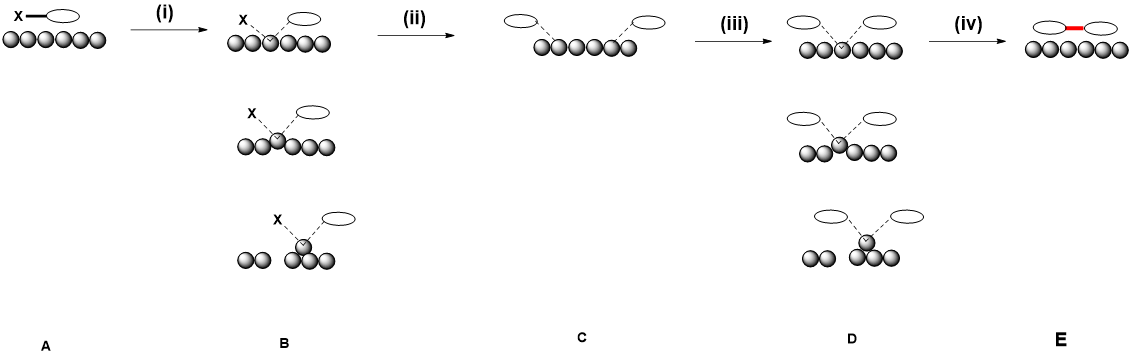
\includegraphics[width=0.48\textwidth]{Fig/mechanism.png}
\caption{Elementary steps of a surface Ullmann Coupling reaction mechanism}
\label{fig_mecha}
\end{figure}
%(ZZ: I suggest we change the mechanism figure here, maybe emphasize the possible intermediates in the text?)

As shown in Fig.~\ref{fig_mecha}, the formation of organometallic intermediates is involved in the process of surface Ullmann coupling, which also appears in the mechanism of solution Ullmann coupling. It is worth tracking the pathway that metal atoms participate in the coupling process. Since all reactants and intermediates are adsorbed on the metal substrate in surface Ullmann coupling, it is apparently that the active metal species come directly from the substrate. However, the face of metal crystal is not a perfect, well-ordered shape in reality, there exits various of defect, adatoms, vacancies, as shown in Fig.~\ref{cyrstal_surface}~\cite{ullmann_49}. Figuring out the effect of these imperfections on the surface Ullmann coupling would consummate the utilization of various surface. Here we will mainly investigate how adatoms participate in surface Ullmann coupling reaction mechanism, details will be discussed in next section.

\begin{figure}[htb]
\centering
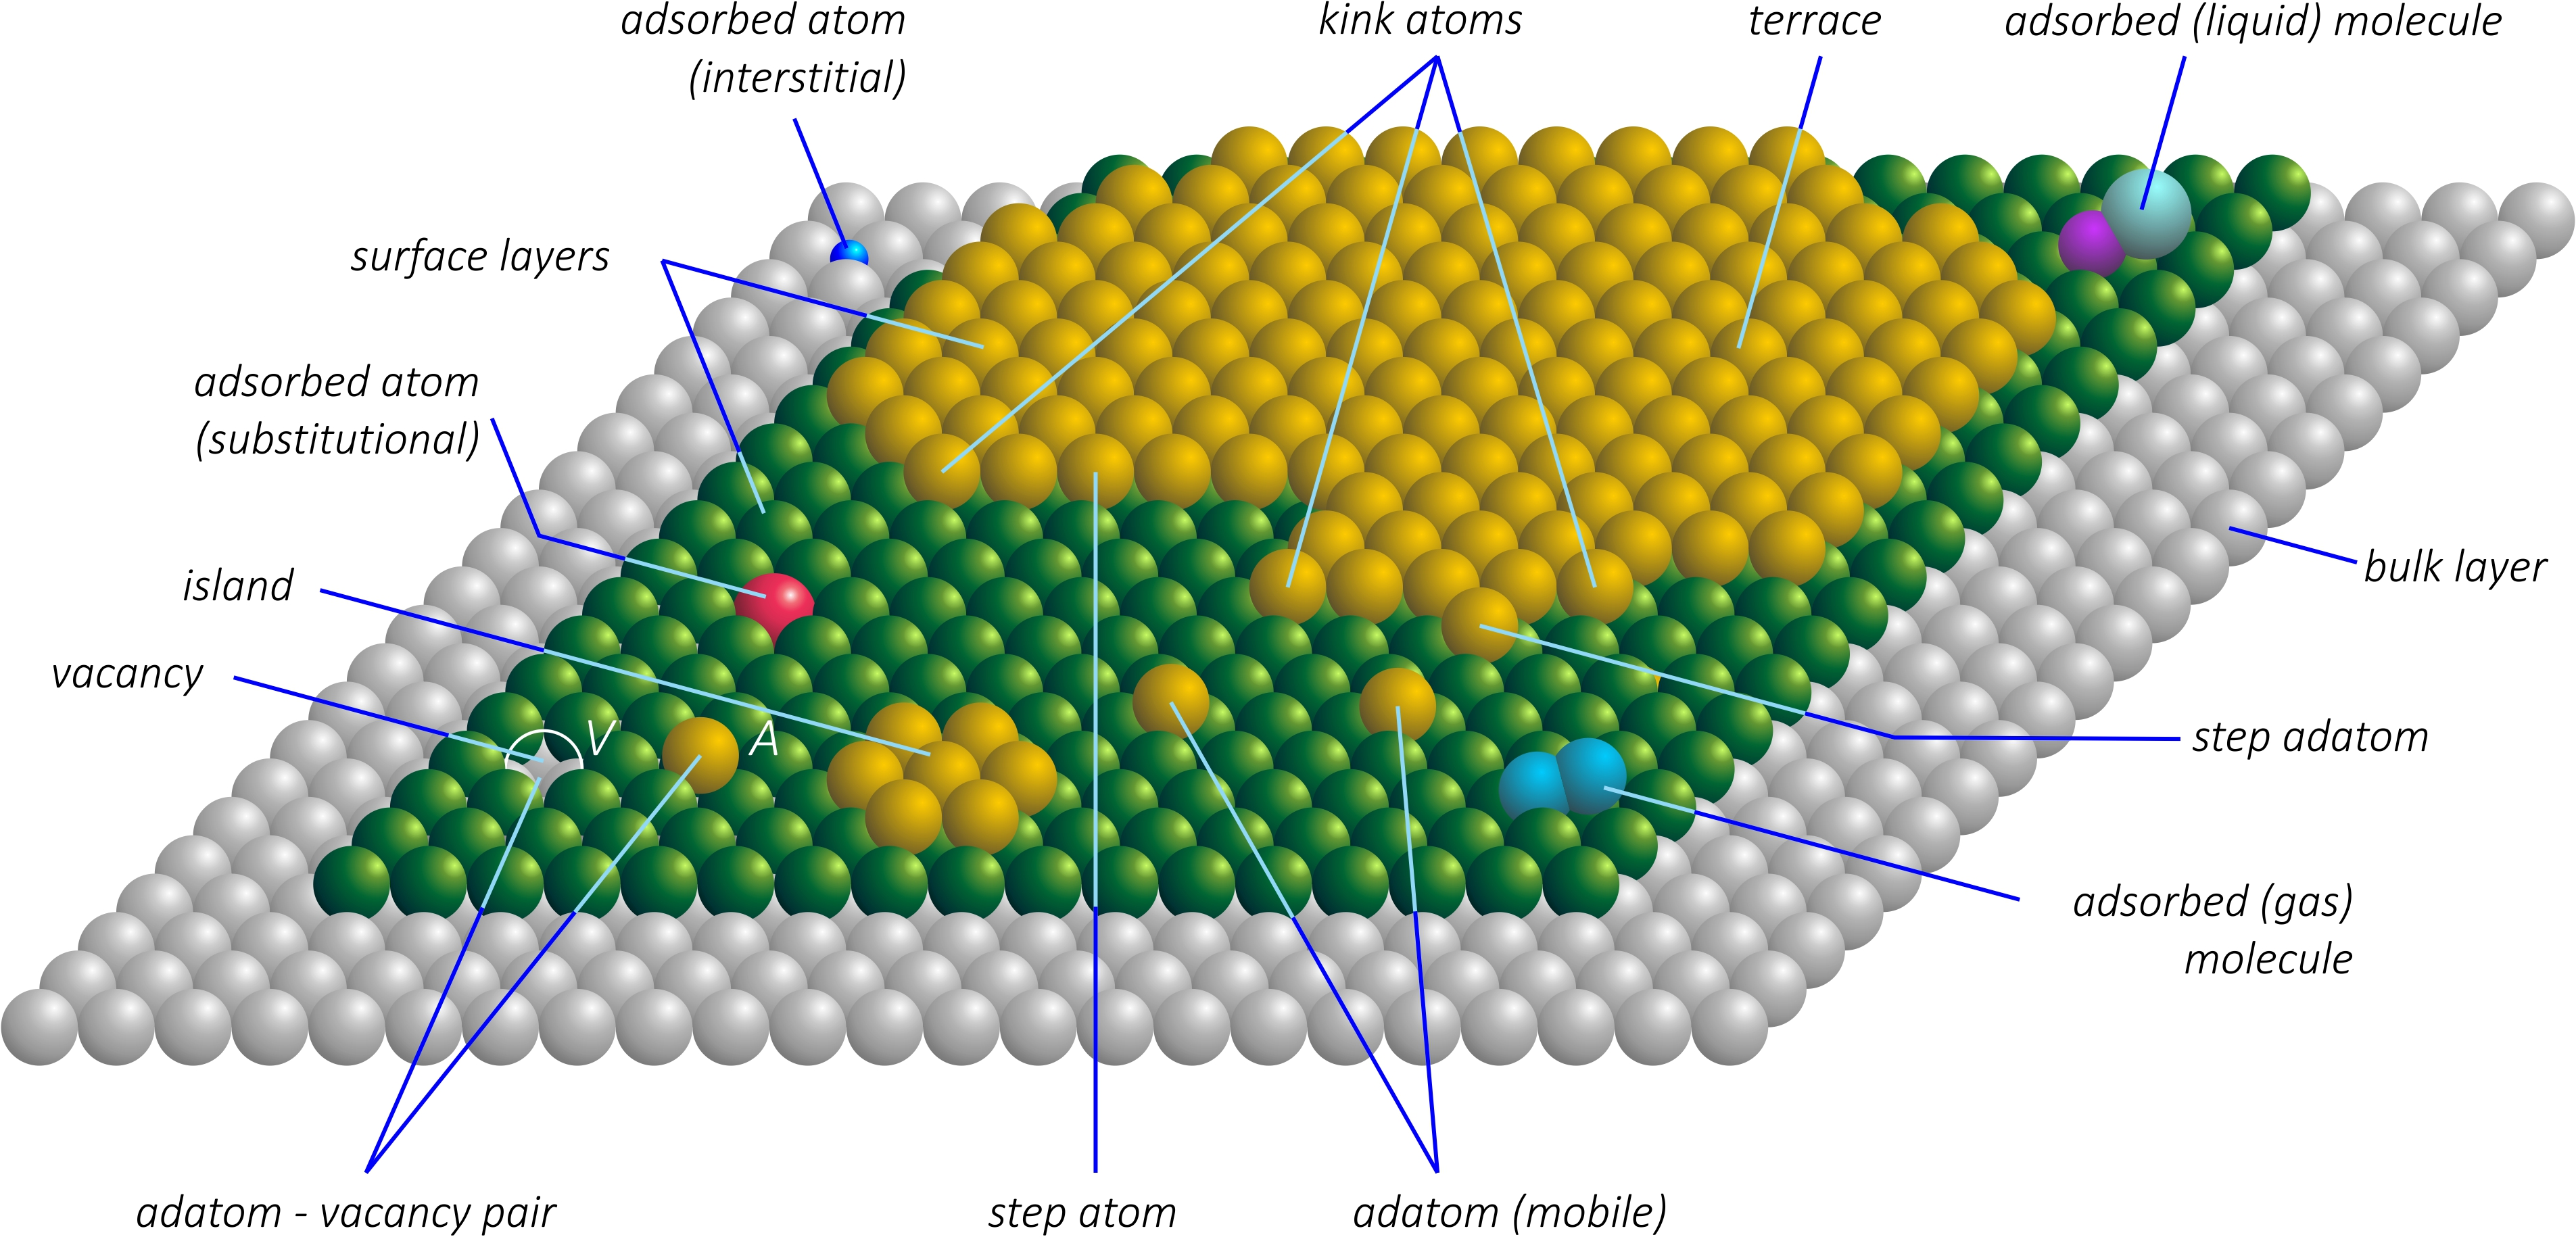
\includegraphics[width=0.4\textwidth]{Fig/Crystal_surface.jpg}
\caption{A model of crystal surface}
\label{cyrstal_surface}
\end{figure}
%%\begin{enumerate}[align=left, itemindent=2em, label=(\roman*)]
    %%\item Dehalogenation of Precursors [The fundamental step is the %%disassociate of halogens, the cleavage of C-X bonds (X = halogens) is %%usually activated by thermal, electron-induced and photon-simulated. %%The energy will vary from 0.05 ~ 0.80 eV with different X on different %%coinage surfaces.]
    %%\item Diffusion of single Dehalogenlated 'Radicals' [The removal of %%halogens from precursors results in unsaturated carbons (radicals), %%which interact with metal atoms to form C-Metal radical (C = %%dehalogenated precursor and Metal = Au, Ag or Cu). C-Metal radical %%will diffuse on metal surface and the metal atom interacting with the %%radical will shift.]
    %%\item The Formation of Organometallic Intermediates C-Metal-C from Two %%Single Radicals [Diffusion brings two single radical close to each %%other, and then these two species would form a dimerized %%organometallic intermediate before the appearance of coupling product]
    %%\item The Formation of Carbon-Carbon Bond []
    %%\item Diffusion of Coupling Product []
%%\end{enumerate}  

\subsubsection{\label{sec:level3}Dehalogenation}

%RZZK: carbon or heteroatom? 
%RZZK: no reference to the figure steps (%ZZ: added)
The first fundamental step of the surface Ullmann coupling is the dissociative dehalogenation of organic precursors adsorbed on the surface. In this step, C--X bonds are broken while carbon-metal and halogen-metal bonds are formed. The thermodynamics and kinetics of the process are primarily determined by the relative strength of the broken and formed bonds. 
Bond strength (X = Halogen):
%RZZK: I did not check the actual strength for these bonds, please check the trends (%ZZ: checked and literature attached)
%
\begin{eqnarray}
\text{C -- Cl} > \text{C -- Br} > \text{C -- I} \\ 
\text{Cu -- C} > \text{Au -- C} > \text{Ag -- C} \\
\text{Cu -- Cl} > \text{Cu -- Br} > \text{Cu -- I}\\
\text{Au -- Cl} > \text{Au -- I} > \text{Au -- Br} \\
\text{Ag -- Br} \approx \text{Ag -- Cl} > \text{Ag -- I} 
\end{eqnarray}
(M-X bond strength is compared according to bond dissociation energy of diatomics~\cite{ullmann_62}, C-X bond strength according to the bond dissociation energy in CX$_4$ molecule~\cite{ullmann_63}, M-C bond strength according to the metal-carbon bond distance in M-(CH$_3$)$_2$~\cite{ullmann_61}).
For surface Ullmann coupling reaction, M-X bond strength can be compared together to present an overall relationship.

\begin{gather*}
\text{Cu -- Cl} > \text{Cu -- Br} > \text{Au -- Cl} \approx \text{Au -- I} \approx \text{Ag -- Br}\\
 \approx \text{Ag -- Cl} > \text{Ag -- I} > \text{Au -- Br} > \text{Cu -- I}
\end{gather*}
%
%RZZK: Experimental trends in the halogen series. Compare observables (for example, dissociation temperature) for X=I,Br,Cl and the same metal (say, Cu). (%ZZ: added)
%RZZK: What of the two factors influence this step more: the nature of the halogen or the nature of the metal? Is it possible to arrange the nine M--X cases in term of bond strength? It is possible to do a whole study on the predicting the energetics of this step based on bond energies. This can be done in the results and discussion, if necessary. (%ZZ: added)
This data also indicate the distinct influence of surfaces, which has been proven in experiment of bromobenzene and iodobenzene. For instance, the dissociaton of iodobenzene occurs at approximately 175~K on Cu(111)~\cite{sur_sci01}, 200~K on Ag(111)~\cite{sur_sci02} and 250~K on Au (111)~\cite{sur_sci03}. The same trend has been demonstrated by bromobenzene with a higher T on all surfaces.

In 2013, Björk \textit{et al.} ~\cite{jacs2013} proposed an activation barrier of 0.4-1.0 eV for exothermic dehalogenation by DFT simulations. In specific, bromobenzene and iodobenzene on Au(111), Ag(111) and Cu(111) surface displayed different reactivity, i.e., the activation barrier and reaction energy both decrease in the order Au $>$ Ag $>$ Cu, and for all surfaces studied, iodine substituent are 0.1-0.5 eV lower than bromine ones in dehalogenation As shown in Fig.~\ref{fig:dehalo}. The trend is plausible due to the Bond-dissociation energy (BDE) of C-I is ~0.65 eV lower than C-Br\cite{Arpc1982}.

\begin{figure}[tbh]
\centering
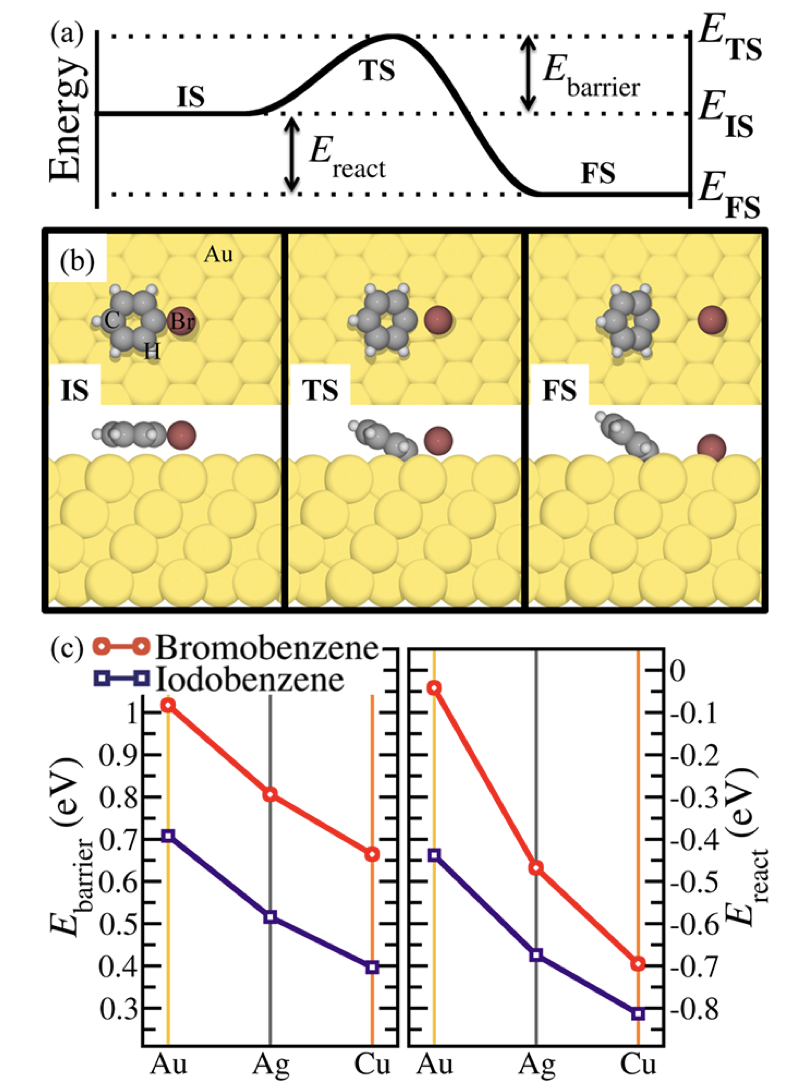
\includegraphics[width=0.75\columnwidth]{Fig/dehalogentaion.png}
\caption{Figure 1. (a) Definitions of the energy barrier ($E_{barrier}$) and reaction energy ($E_{react}$) for dehalogenation reactions. (b) The dissociation of bromobenzene on Au(111), depicting top and side views of the initial state (IS), transition state (TS), and final state (FS) of the reaction. (c) $E_{barrier}$ (left) and $E_{react}$ (right) for the dissociation of bromobenzene and iodobenzene on the (111) facets of Au, Ag, and Cu.} 
%RZK: Detailed description of the figure. Take a look at the original publication. Reprinted from~\cite{RZK} with permission of American Chemical Society or PUBLISHER. See the LaTeX comment below.
%%RZK: If you take a figure from a publication it is very important to cite the work and obtain publisher's permission. We need to make sure that all our borrowed figures satisfy copyright permissions. For example, see: https://www.stm-assoc.org/2016_01_05_Guidelines_for_Quotation_From_Journal_Articles.pdf (%ZZ: need to discuss)
\label{fig:dehalo}
\end{figure}

%RZZK: diffusion of halogen atoms? (%ZZ: added)
%RZZK: dissociation products?(%ZZ: added)
\subsubsection{Diffusion of unsaturated carbon species on surface}

%RZK. Compare the two versions.
The dehalogenation step produces unsaturated carbons species(surface-stabilized single radicals), the dangling bonds of this unsaturated carbons bind to the adjacent metal atom. The diffusion of this  unsaturated carbon species, or phenyl groups play a decisive role in further coupling process. 
%The dehalogenation step produces organometallic intermediates with carbon atoms covalently bonded directly to surface metal atoms. On the next key step, these intermediates approach each other by diffusion. 
%
% RZK: note that I use phenyl GROUPS, not RADICALS. (ZZ: solved) 
The diffusion process of phenyl groups have been observed experimentally and studied computationally. A STM imaging has revealed that dehalogenated phenyl groups diffuse on Cu(111) at 77~K~\cite{langm01}. The calculated energy barrier of phenyl groups' diffusion was $\sim$0.09~eV. It has also shown that phenyl groups, which were tilted at $\sim 36^\circ$ with respect to the surface~\cite{pccp2010}, overturn during the diffusion and then bind to a nearby metal atom as shown in Figure.~\ref{fig:4}. This was also discussed by Björk \textit{et al.}~\cite{jacs2013}. Phenyl was proposed to diffuse either by sliding or flipping. In sliding fashion, phenyl stayed the same orientation in initial state and final state, the energy barriers of diffusion on different metal surface followed the order: Cu(111) $>$ Ag(111) $>$ Au(111). While in flipping pattern, the order of diffusion barriers changed to Au(111) $>$ Cu(111) $>$ Ag(111). Since the flipping pattern on these metals all possessed a lower energy barrier for diffusion, it was considered as a more plausible fashion for phenyl to diffuse on metal surfaces. Overall the ease diffusion will increase the possibility that two single phenyl groups move closer to each other, which can result in the further dimerization of them.
%RZK: Are their any trends in the diffusion activation barriers for different metals? (%ZZ: Added a comparison.)
Besides the phenyl groups, halogens are also dissociated from the original precursors and chemisorbed by the surface metal atoms. In 2013, Björk \textit{et al.}~\cite{jacs2013} investigated the binding energy and the diffusion barrier of dissociated halogens on metal surface using DFT calculations. Bromine and Iodine atoms will both display a mobility at experimental temperature due to a small diffusion energy barrier in the range of 50-100 mv on Cu(111), Ag(111), and Au(111). The barrier is largest on Au(111) while smallest on Cu(111). Although halogens are free to move, they possess a relatively high binding energy to metals. The smallest binding eneryg is halogens on Au(111), around 2.80 eV and the highest is on Cu(111), around 3.1 eV, which indicate that the halogens are even harder to desorped than those dehalogenated phenyl groups. Research also showed that the halogens remained on metal surface will further hinder the diffusion, coupling and polymerization of phenyl groups~\cite{ullmann_64,ullmann_65}. Removing the byproducts of on-surface Ullmannn coupling is also of great significance.

\begin{figure}[htb]
\centering
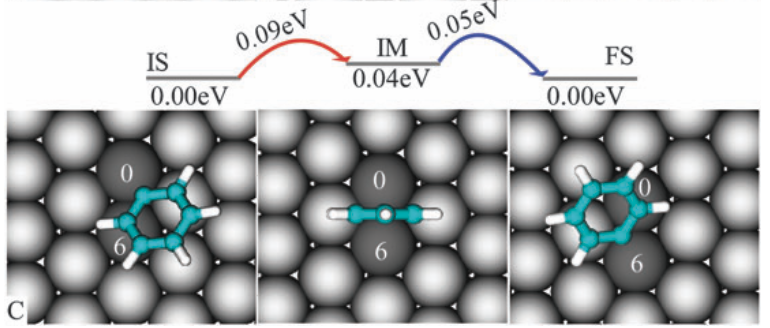
\includegraphics[width=0.75\columnwidth]{Fig/overturn.png}
\caption{Diffusion of phenyl group on Cu(111): phenyl group migrates from Cu0 to the neighboring metal atoms} %RZK: better caption, copyright. (%ZZ: added)
\label{fig:4}
\end{figure}

%RZZK do we need to keep the following or is it too obvious?: The diffusion energy barrier and the tilt angle between single radical and substrate will change with the size increasing of reactant molecules.(%ZZ: True, I think we don't need to mention this)

%RZK: What happens to halogen atoms? How mobile are they? A couple of sentences. (%ZZ: I think we could describe this in our result section? cause we have the results)

\subsubsection{Formation of dimerized organometallic intermediates}

%RZK: "close" or do they have to be bonded to the same metal atom? (%ZZ: solved)
A dimerized organometallic intermediate based on carbon-metal-carbon interlinks forms when two single phenyl groups diffuse adjacent to each other and then interact with the same metal atom. These carbon-metal-carbon bridges have been revealed in related research works. 

In 2011, Wang \textit{et al.}~\cite{jacs2011} studied the organometallic intermediate of surface Ullmann coupling from dibromoterphenyl to polyphenylene using STM and DFT calculations. When the temperature went to 300 K, both Br atoms were dissociated from the phenyl group. However, the length of linear periodic structure formed in reaction (characterized by STM) was 4.8 \AA\ longer than the length of DFT calculated terphenyl group (ph)$_{3}$, which indicated the possibility that copper atoms were inserted and served as linkage parts inside terphenyl groups. Besides, performed tunneling spectra (dI/dV) of one periodic unit of the experimental formed structure and the calculated projected density of states (PDOS) of (ph)$_{3}$/Cu atom both showed the same value at ~2.7 eV, which further proved the existence of C-Cu-C bridges in organometallic intermediate structures, all the evidences are shown in Fig.~\ref{fig:organ}. Similar methods have been used by Chung \textit{et al.}~\cite{PCCP2012} with the same molecules on Ag(111). C-Ag-C bridges were observed and demonstrated in the organometallic intermediates.

The C-Ag-C and C-Cu-C structures were both obtained at 300 K, which revealed that the barrier for two terphenyl
coordinated with Ag and Cu are close. Compared to the dehalogenation, this step requires a higher temperature condition (still near room temperature). On Cu and Ag surface, the dimerized organometallic intermediates are always observed, but on Au surface are occasionally reported. This is explained by a relatively low barrier conversion from this state to covalent bond formation on Au surface, resulting in a very short life time of C-Au-C existence~\cite{ullmann_33}.
%
\begin{figure}[ht]
\centering
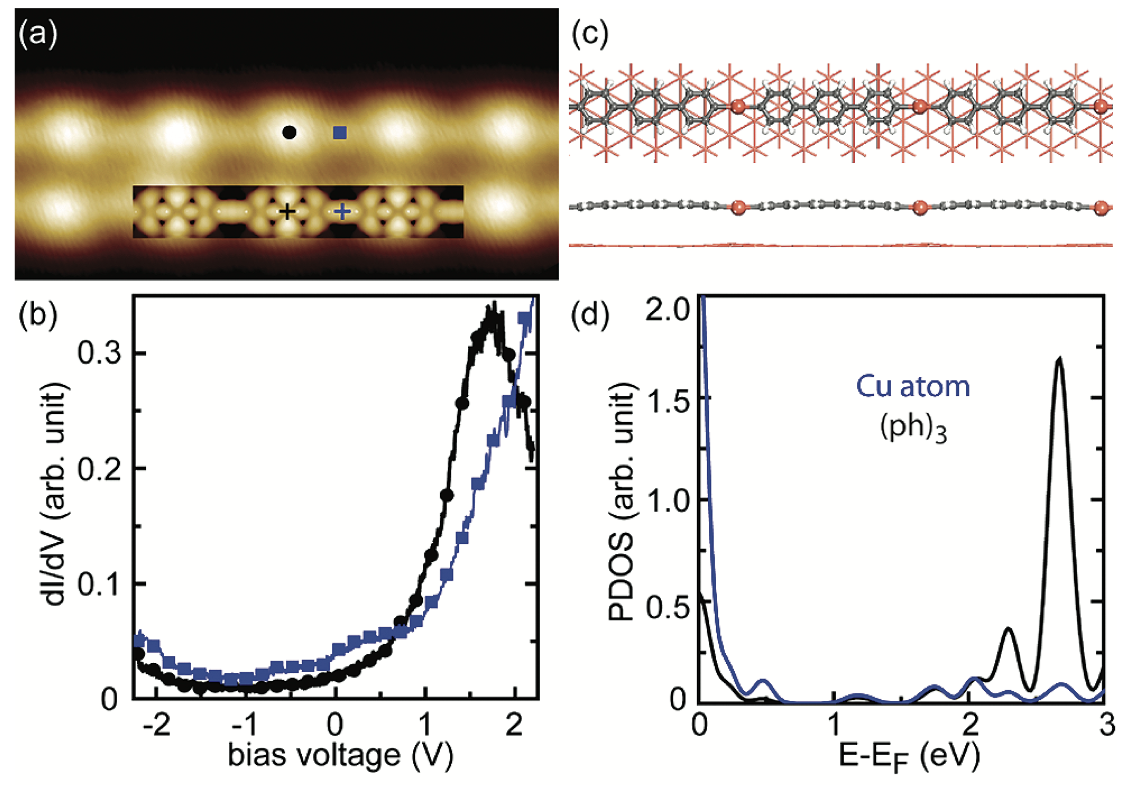
\includegraphics[width=0.75\columnwidth]{Fig/Organometallic.png}
\caption{(a) High-resolution STM image of the intermediate (8 $\times$ 4 $nm^2$, 1.0 V, 0.5 nA). (Inset) Simulated STM image at +2.7 V on the same scale. (b) dI/dV spectra measured at (ph)$_3$ (black dot) and Cu atom (blue square) sites as marked in (a). (c) Top and side views of the optimized structure of the intermediate obtained by the DFT calculation. (d) Calculated PDOS of (ph)$_3$ unit (black) and Cu atom (blue) as marked by the crosses in (a).}
\label{fig:organ}
\end{figure}

\subsubsection{Formation of the C--C bond}

%RZK: it is not clear when you describe calculations and when you describe experiments. (ZZ: solved)
%RZK: There are lots of symbols that are not displayed correctly in a pdf. (ZZ: solved)
After further annealing, the metal atoms are released from the dimerized organometallic intermediates, spontaneously a covalent bond will be irreversibly constructed between two carbon atoms. The formation of C--C bond in this state has also been widely explored in experiment and theoretically as well. In 2016, Di Giovannantonio \textit{et al.}~\cite{jacs2016} reported the dimerization and trimerization of 1,4-dibromobenzene on Cu(100) in UHV condition and related simulations with DFT methods. DFT results predicted that the dimerized organometallic intermediate was a relatively stable phase in potential energy surface. A 0.7 eV of activation energy was required from the dimerized organometallic intermediate to the coupling dimer. And a 0.2 eV of activation was needed for the coupling dimer to produce the trimer product, the data could be reviewed in Fig.~\ref{fig:dimer}. These data are consistent with Di Giovannantonio's another experiment work~\cite{acsnano2013} in 2013. Same precursor 1,4-dibromobenzene was deposited on Cu(100) surface and the surface Ullmann coupling process was pictured in STM image. It was reported that organometallic intermediates were formed at room temperature, nevertheless the final formation of C--C bond needed an annealing temperature up to 500 K.
%
\begin{figure*}[ht]
\centering
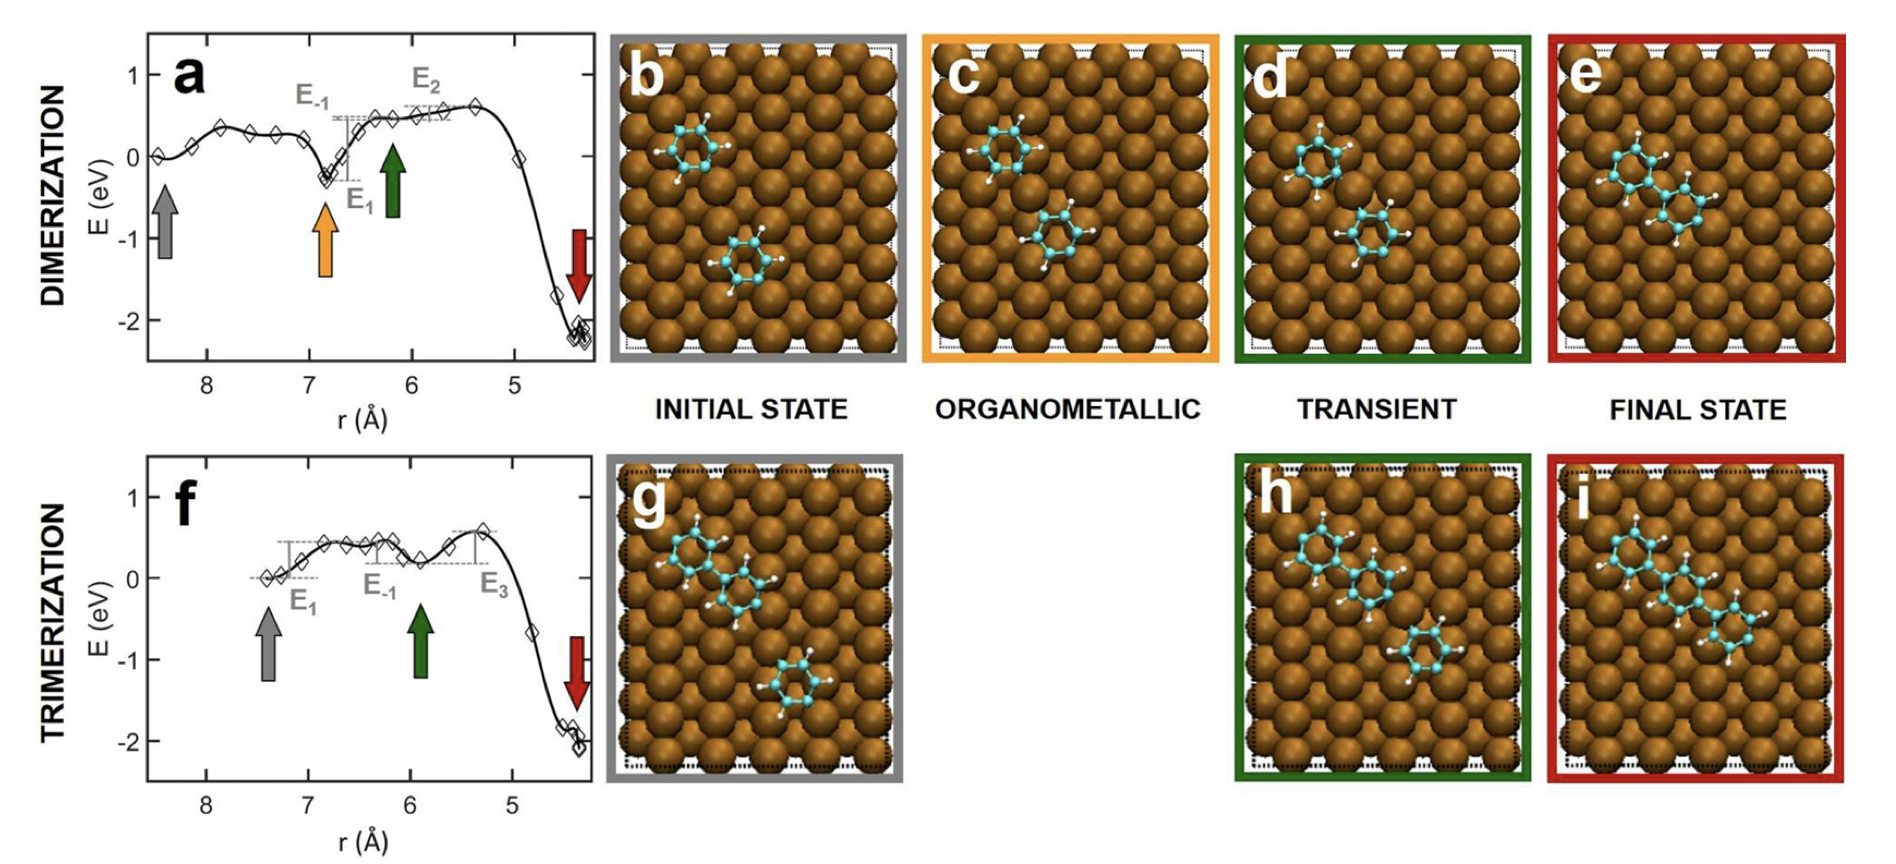
\includegraphics[width=1.0\textwidth]{Fig/Dimer_trimer.png}
%R1111: What metal is this. Better captions are required for all figures. Chemical identity of all species must be clear from the figure.
\caption{Coupling barriers between (a) two monomers (dimerization) and (f) a monomer and a dimer (trimerization), respectively. The length (r) indicated in angstrom is the distance between the centers of the aromatic rings which undergo covalent coupling. The geometries of the most significant states (initial, organometallic intermediate, transient, and final) are reported in panels b−e and panels g−i for the dimerization and trimerization, respectively. The colors of the frames correspond to the arrows in panels a and f.}
\label{fig:dimer}
\end{figure*}
%

This final step requires a higher annealing temperature, range from 330 to 420 K on Ag surface and from 500 to 600 K on Au surface~\cite{ullmann_51}, and on Cu, the temperature range is usually lower than on Au but higher than on Ag. This indicates that the energy barrier of the formation of C--C bond step on three metal surfaces should follow Au $>$ Cu $>$ Ag. And since  there were limited reports on the formation of C-Au-C intermediates, it could be safely speculated that a high energy barrier exists in the formation of C-Au-C dimerized organometallic intermediates and a low barrier exists in the  covalent bond formation. After the formation of C--C bond, a surface Ullmann coupling would be completed between two monomers, resulting in a dimer. If there are more than one functional group on a monomer, this dimer could further diffuse and couple to obtain a trimer~\cite{jacs2016}, and oligomer~\cite{ullmann_53, ullmann_56} or polymer~\cite{ullmann_43, ullmann_54, ullmann_55}.

\subsubsection{Summary on mechanism of surface Ullmann Coupling}

Overall, the effect of halogens and metal types on each step of surface Ullmann coupling reaction mechanism have been exhaustively explored. 

On dehalogenation step, it has been shown that the reactivity trend follows the order Ar-I $>$ Ar-Br $>$ Ar-Cl both in experiment and theoretically~\cite{ullmann_52}. This also means that the dissociation of Ar-I bond on metal surface requires the lowest temperature. In addition, the energy barrier of dehalogenation is the highest on Au(111) surface, the lowest on Cu(111) surface both in experiment and in theoretical calculations~\cite{jacs2013}. It also reported that the miller index of metal surface would also make a difference here~\cite{ullmann_57}. 

Then considering the next step, it has been discussed that the diffusion of phenyl group on Au(111) surface is the most energetically favorable, while on Ag(111) is the least. The halogens are supposed to have little influence on the diffusion step, but it might hinder the two phenyl group to diffuse close to each other. 

When it comes to the formation of dimerized organometallic intermediates, it was concluded that C-Au-C structure is the hardest to obtain, the construction of C-Ag-C and C-Cu-C should have close energy barrier due to the similar temperature condition of this step in experiments. 

The covalent bond formation is the last step, it has been mentioned that the C--C bond construction required least energy on Ag surface while highest on Au surface.  

\subsection{Role of adatoms in the surface Ullmann coupling} 

Metal atoms are involved in many steps of the mechanism of surface Ullmann coupling reaction discussed above. Investigation into the role of metal atoms in this process delivered a long-existence argument.
%%%%%%%%%%%%%%%%%%%%%%%%%%%%%%%%%%%%%%%%%%%%%%%%%%%%%%%%%%%%%%%%%%%%%%%%%%
%%The metal atoms may come from: (1) adatoms residing on metal surface; %%(2) metal atoms reside inside the metal surface. These two possibilities %%have been explored both experimentally and computationally in first %%three steps. \\
%%%%%%%%%%%%%%%%%%%%%%%%%%%%%%%%%%%%%%%%%%%%%%%%%%%%%%%%%%%%%%%%%%%%%%%%%%
Here the two terminology $Nature$ and $Origin$ will be used to distinguish the metal atoms which participate in suface Ullmann coupling.
The %Nature% of metal atoms means metal atoms can come from (1) surface atom which is located at the first layer on metal surface, is indistinguishable from other surface atoms and has no relation with surface defect, or (2) adatoms which is related to the surface defect, it will lie above the first layer of metal surface and free to diffuse.
Thus, the $nature$ mainly divide the metal atoms from a surface into two categories, the first kind is indistinguishable and locate in the lattice of metal crystal, while the second kind is adatoms, which is a production of common non-order defect appeared on metal surface. 
The process that gives birth to $nature(2)$, adatoms in surface Ullmann coupling reaction is also of great interest. It can be split into two different kinds with notation $origin$: adatoms in surface Ullmann coupling may come from (1) pre-exsiting adatoms before the occurrence of surface Ullmann coupling due to the surface defect, thermal punctuation or (2)pulled out by the intermediates produced in surface Ullmann coupling, and then fully sit above the first layer of metal surface to become a new adatom. For the second origin of adatoms, it can also be expressed that the surface Ullmann coupling create this adatom which used to be a $nature(1)$ atom. The nature of metal atoms and the origin of adatoms have been explored experimentally and computationally.
%For origin(1), it has been reported that the onset of the vacancy-adatom formation take place on Cu(111) surface was around 900 K by molecular dynamics~\cite{ullmann_50} , which is much higher than the temperature required by surface Ullmann coupling reaction, as shown in Fig.~\ref{fig:2Dgasn}~\cite{ullmann_50}. This could be the evidence that there would not be new adatoms formation due to the thermal fluctuations as the surface Ullmann coupling proceeds. 

%discuss that adatoms could exit on metal surface due to the thermal evaporation
For $origin(1)$, it has been explored that the number of mobile adatoms on copper surface are high at room temperature~\cite{ullmann_58}, especially near various surface defect, which provide a feasible view that the formation of organometallic intermediates in surface Ullmann coupling may directly make use of $origin(1)$ adatom. Thus, it is safely suspected that there is an comparison between $nature(1)$ and $nature(2)$ metal atoms which will be made use of in the process of surface Ullmann coupling reaction and also decide whether surface Ullmann coupling reaction will be a method to create $origin(2)$ adatoms in experiment. These possibilities are detailed discussed in following sections.





%\begin{figure}[ht]
%\centering
%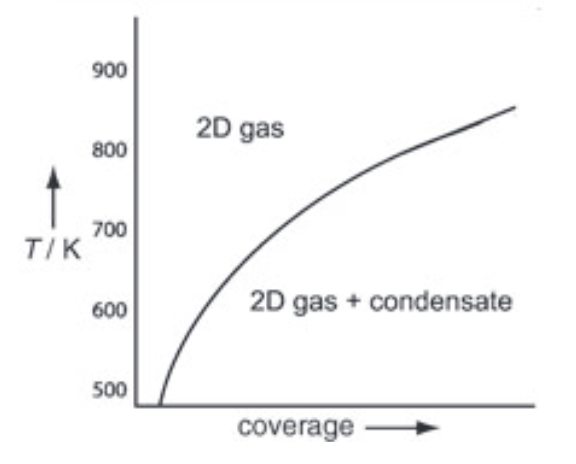
\includegraphics[width=0.75\columnwidth]{Fig/2D-gas.png}
%\caption{Schematic diagram of 2D adatom gas phase and condensed phase (islands) %coexisting at elevated temperatures for metal-on-metal systems.}
%\label{fig:2Dgas}
%\end{figure}

\subsubsection{\label{sec:level3}Dehalogenation of precursors}

Evidences have already been presented that metal adatoms participate in the process of dehalogenation. 
In 2017, Barton \textit{et al.}~\cite{chemeurope2017} explored the role of adatoms in the dehalogenation step with iodobenzene on Au(111), Ag(111) and Cu(111) surface based on DFT calculations. The energy profile of adatom formation on pristine surface was compared with the profile of formation on surface with the presence of iodobenzene, the latter case is referred to as adatom formation of $origin(2)$. The comparison has shown that the energy of extracting a metal atom from the pristine surface was in the 1.12 - 1.71~eV range. While in the dehalogenation step, the dehalogenated iodobenzene would interact with the metal atom of $nature(1)$ on metal surface, which would possibly form a new adatom of $origin(2)$. This step required a dramatically lower energy of 0.16-0.60~eV range. Furthermore, the calculations have shown that the energy released in the process of adsorption of idobenzene on metal surface and formation of organometallic intermediates in the process of surface Ullmann coupling is sufficient to compensate the energy required for a metal atom extraction to form a new adatom of $origin(2)$, as shown in Fig.~\ref{fig:3}.
\begin{figure}[htb]
\centering
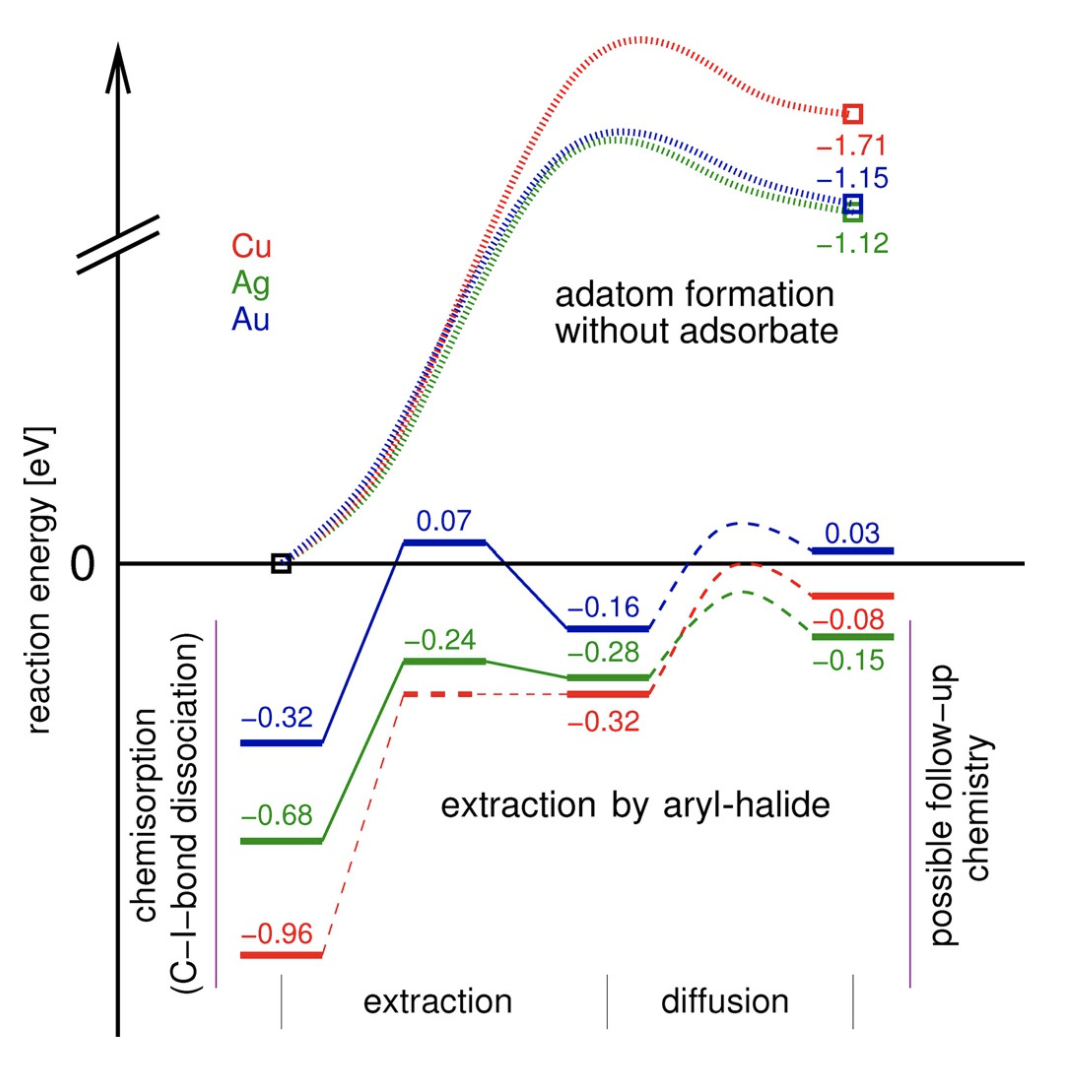
\includegraphics[width=0.75\columnwidth]{Fig/Adatom-formation.png}
\caption{Graphical comparison of the energetics of the adatom formation without adsorbate (top half) to the extraction by aryl–halide process (lower half).Values for Cu are shown in red, for Ag in green and for Au in blue. The extraction-by-arylhalide process starts from the dissociated iodobenzene. Dotted lines indicate parts of the energy profile that have not been quantitatively resolved.}
\label{fig:3}
\end{figure}

It is clear that metal atoms of $nature(1)$ have a great chance to participate in dehalogenation, the first step of surface Ullmann coupling. And the construction of organometallic intermediate in the dehalogenation could possibly be a feasible pathway to form adatom of $origin(2)$. Metal atoms of $nature(2)$ in the dehalogenation had few related reports to date.

\subsubsection{Diffusion of two dehalogenated phenyl groups}

The diffusion process is involved in the interaction between single precursor group and metal atom. 
In 2018, Nagoya \textit{et al.}~\cite{jpcc2018} investigated the mechanism of Ullmann coupling of 7,10-dibromofluoranthene (Br$_{2}$FL) on Au(111) via DFT calculations. Compared to simple phenyl rings that tend to form ~$36^\circ$ tilt angle with Cu(111) surface~\cite{pccp2010}, the monobromo FL with one Br atom removed would stay almost parallel to Au(111) surface due to steric repulsion between the large backbone of BrFL group and the substrate. And BrFL group was found to lift surface Au atom out by 1.9 \AA\ from its initial position, which is much larger than 0.16 \AA\ height lifted by a simpole phenyl ring, as shown in Fig.~\ref{fig:diff}.
Ebeling \textit{et al.}~\cite{acsnano2019} also indicated 4-bromo-3$^{''}$-iodo-$p$-terphenyl group interacts with the Cu atom inside the surface, and would partially lift the Cu atom out from the surface while diffusing on Cu(111) surface. 
\begin{figure}[hbt]
\centering
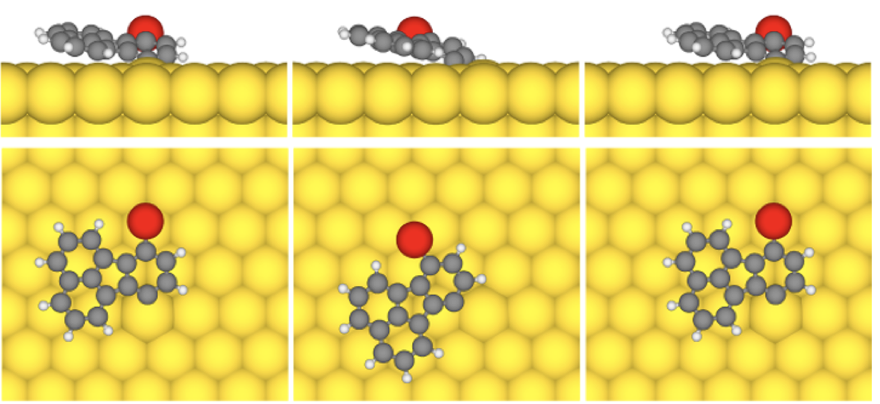
\includegraphics[width=0.75\columnwidth]{Fig/Diffusion_path.png}
\caption{Top and side view of the initial, transition and final geometries of BrFL molecule diffuse.}
\label{fig:diff}
\end{figure}

Metal atoms of $nature(1)$ were proven to play a significant role in the diffusion of dehalogenated phenyl groups, the metal atoms that interact with phenly groups will be partially lifted from its original position, the lifting height is affected by the intensity of interaction between the phenyl group and metal atom. Formation of adatom of $origin(2)$ has not been reported in diffusion, which indicates that the interaction between phenyl group and metal atom in this step is not in the magnitude to fully extract a metal atom of $nature(1)$. 

\subsubsection{Formation of dimerized organometallic intermediates from two precursor groups}

The nature of the metal atoms in dimerized organometallic intermediate has been investigated through multiple approaches. Besides, it can be deduced that an metal atom of $nature(2)$, which is also an adatom of $origin(1)$ will exit above the first layer of surface before the surface Ullmann coupling reacion occurs. And this atom can attract two phenyl groups diffuse close to it and form the dimerized organometallic intermediate in this step. This type of formation might require less energy compared to the situation that two phenyl groups both interact with the same metal atom of $nature(1)$. The arguments on the nature and origin of metal atoms in this step are intense in the mechanism of surface Ullmann coupling.

In 2017, Zint \textit{et al.}~\cite{acsnano2017} analyzed structures of intermediates in the polymerization of bromotriphenylene to bistriphenylene on Cu(111) surface using STM, AFM image and DFT calculations. Two computational models were compared: two triphenylene molecules bonded to an fully-out-of-surface adatom (a metal atom of $nature(2)$) and two precursors bonded to an atom partially lifted from Cu surface (a metal atom of $nature(1)$) as shown in Fig.~\ref{fig:5}. It has been concluded that the structures observed in AFM were more consistent with computational adatom ($nature(2)$) models. In particular, the C--C distance in organometallic intermediate was of 3.9 \AA\ measured by AFM, which was closer to the Cu adatom ($nature(2)$) model (3.86 \AA) compared to the partially-lifted Cu atom ($nature(1)$) model (3.42 \AA). Furthermore, the energy for formation of the adatom-containing intermediate from distant precursors was 1.74~eV lower than that of the intermediate with a partially lifted atoms. 
\begin{figure}[hbt]
\centering
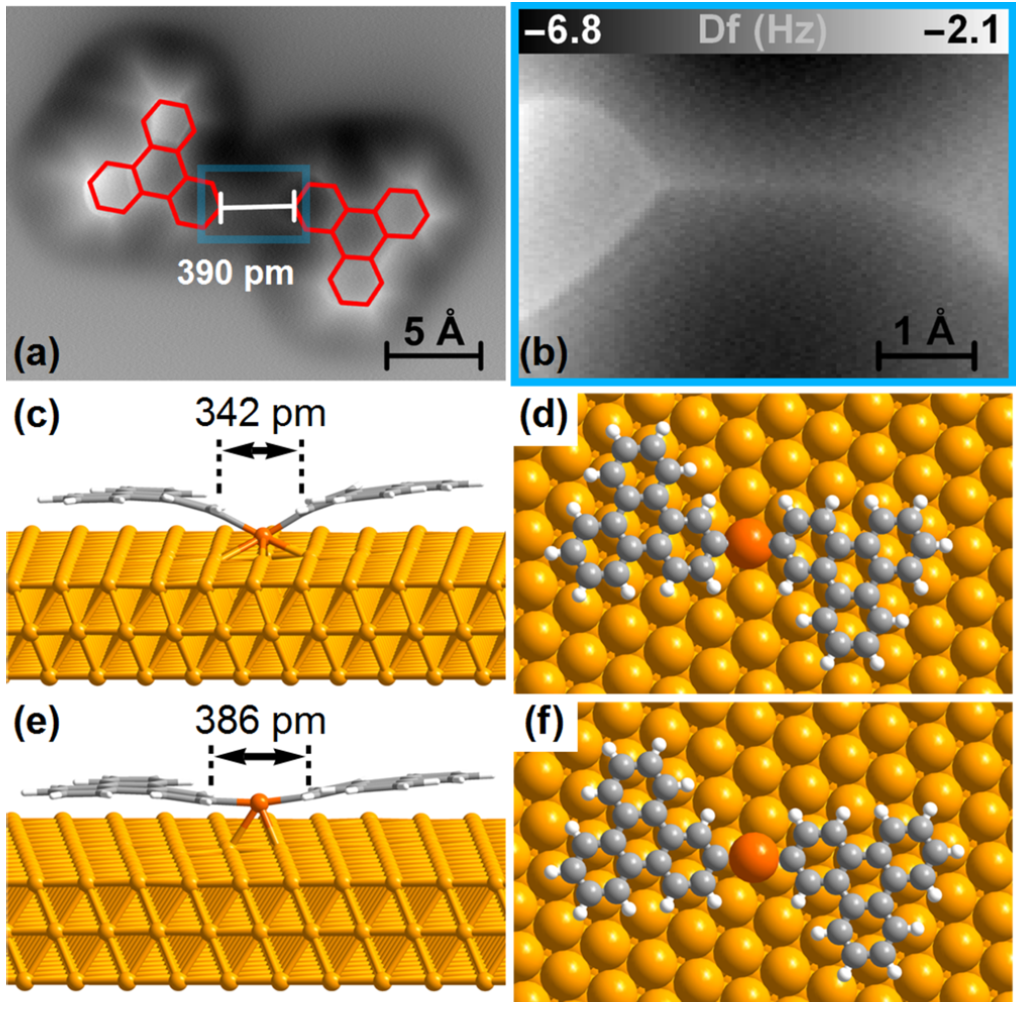
\includegraphics[width=0.75\columnwidth]{Fig/distance.png}
\caption{(a) AFM frequency shift image of intermediate with fit of structural model. (b) Zoom on intermediate bond ($cf$. blue box in a) imaged with decreased tip−sample distance ($\Delta$z = −70 pm with respect to image a). (c−f) DFT-D3 calculations [PBE-D3/ pw (PAW P)] for two different organometallic intermediate states (surface atom (c,d) vs adatom (e,f)).}
\label{fig:5}
\end{figure}

%%ZHZH Dima suggests partial lifting should be discussed separately.
The origin the adatoms were later explored after the metal atoms in dimerized organometallic intermediates were proven to be of $nature(2)$, which is an adatom on surface. In 2019, the study of 4‐Bromo-3$^{''}$- iodo‐$p$‐terphenyl coupling on Cu(111), proved again that the Cu atoms in dimerized organometallic intermediates were adatoms (metal atoms of $nature(2)$) compared experiments with simulated AFM image[Fig.~\ref{fig:6}~\cite{acsnano2019}]. It was further suggested that these adatoms are generated by the extraction of two close single precursor groups (adatom of $origin(2)$), instead of pre-exsiting adatoms (adatoms of $origin(1)$) from a statistic study of all intermediates species in the surface Ullmann coupling.
%
\begin{figure}[ht]
\centering
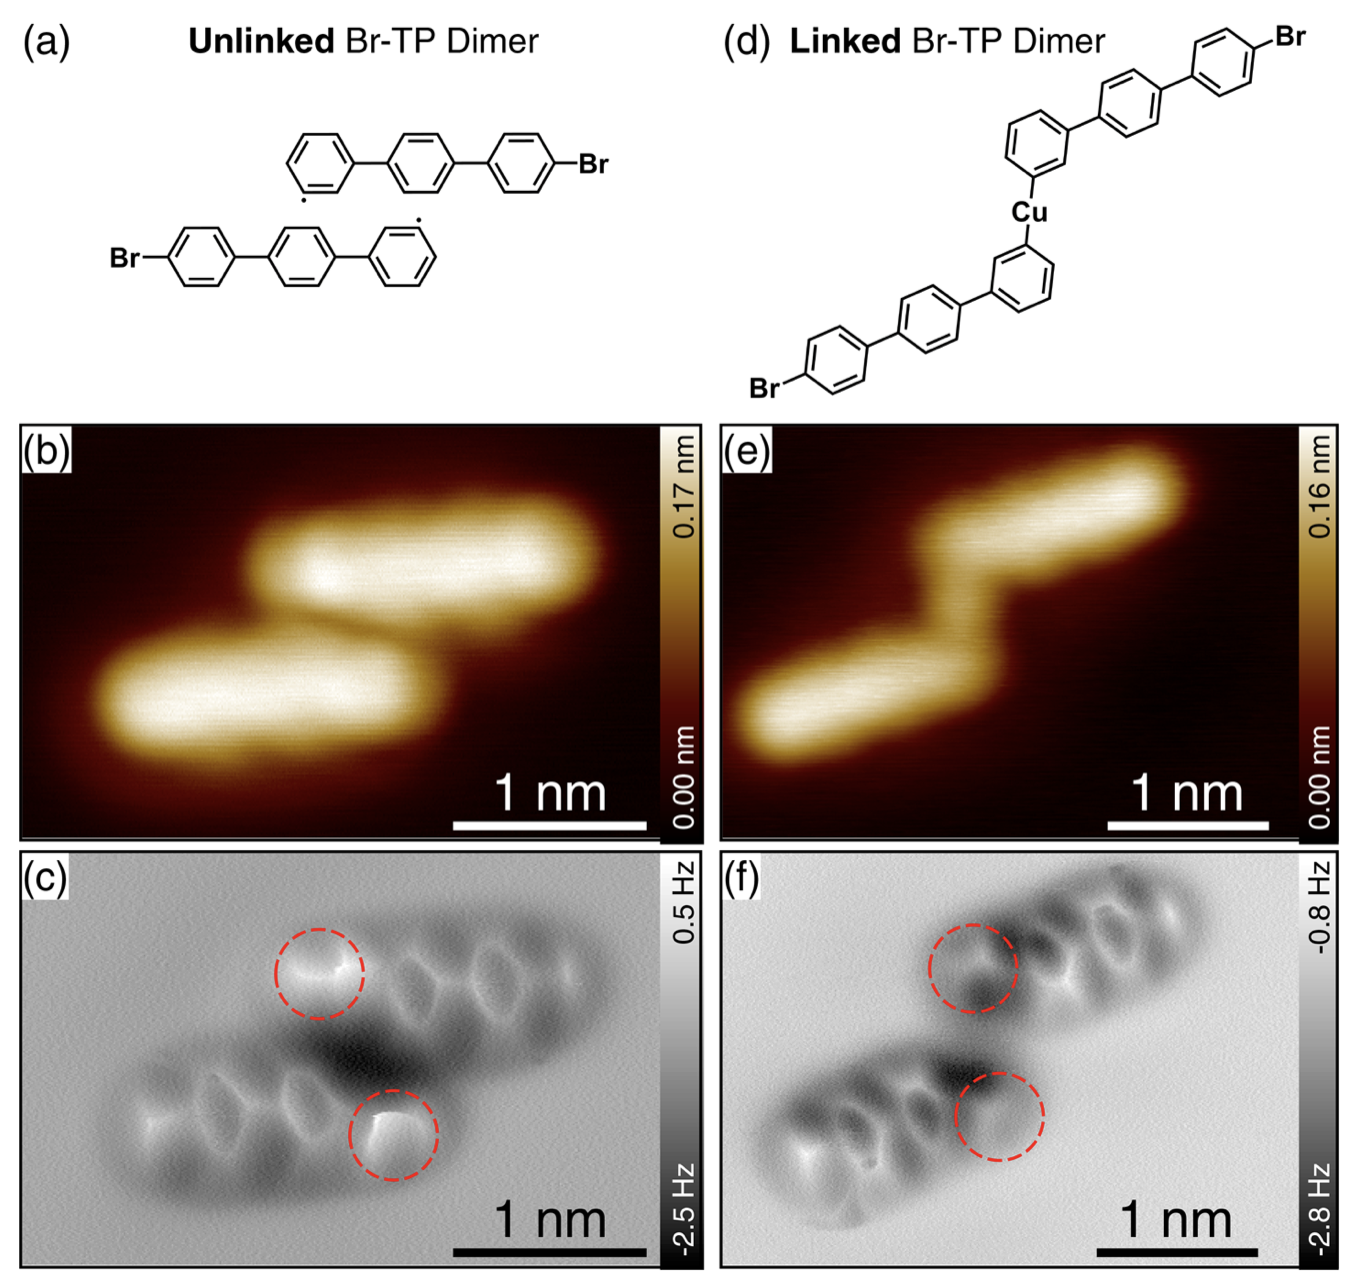
\includegraphics[width=0.75\columnwidth]{Fig/AFM_prove.png}
\caption{Molecular structures (top row), STM (middle row), and AFM images (bottom row) of 4‐Bromoterphenyl dimers on Cu(111). Two different types of dimers are observed, which are denoted as unlinked (left column) and linked dimers (right column). The STM image of the unlinked dimer reveals a dark region between the two molecules that separates them. Between the two molecules of the linked dimer a bright protrusion is observed in the STM scan that directly links them. The red dashed circles in (c) and (f) indicate the twisted phenyl rings, which lost their iodine atoms. Imaging parameters: (b) 200 mV, 30 pA, (e) 200 mV, 10 pA, tip height z = −100 pm (c) and z = −24 pm (f) with respect to a tunneling set point of 200 mV and 10 pA on Cu(111).}
\label{fig:6}
\end{figure}

The nature of metal atoms in dimerized organometallic intermediates has been proven to be an adatom. And further the origin of this adatom is of $origin(2)$, which indicates before the surface Ullmann coupling reaction occurs, the adatom is still a metal atom of $nature(1)$, stay in the first layer of metal surface. After it was selected from two phenyl groups in coupling procedure, it will be fully lifted out of the surface, become a new adatoms. The effect of metal atom in the last step --- formation of C--C bond was not investigated intensive compared to previous steps.

%In addition, chlorinated prophyrin as precursor has also been deposited on Cu(111)~\cite{chematerial2019}. Based on DFT calculations, the Cu adatom mediated path is 3~eV lower than the direct dechlorination. And from STM image, some precursors are still intact at temperature of 400~K, which should be already dehalogenated at lower temperature. It proves that the Cu adatoms are the limiting agent [Fig.~\ref{fig:prophyrin}].

%\begin{figure}[ht]
%\centering
%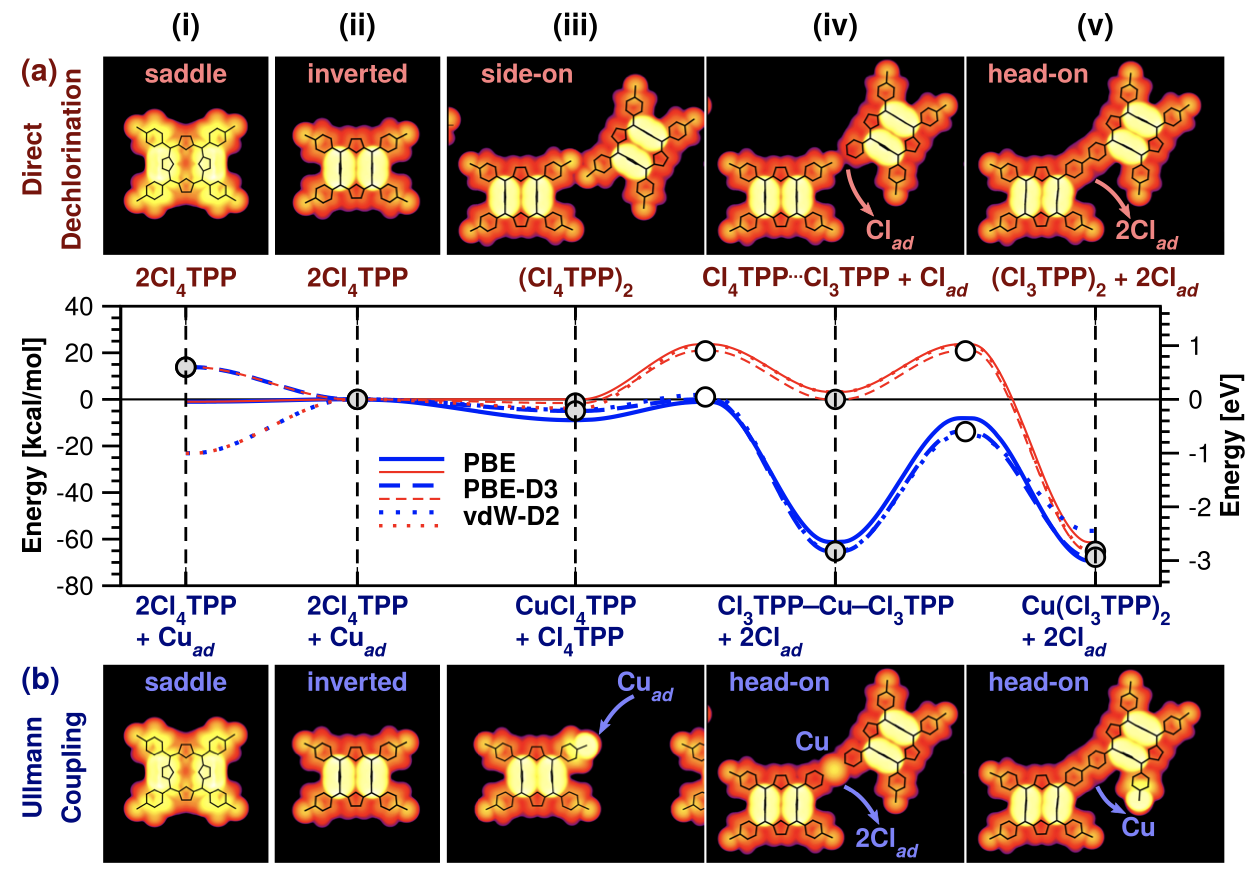
\includegraphics[width=0.4\textwidth]{Fig/Complete.png}
%\caption{STM simulations and DFT reaction profile for the (a) direct %dechlorination reaction (red lines) and (b) Cu adatom-mediated Ullmann coupling reaction (blue lines). For each process the energy are plotted of the (i, ii) precursors, (iii, iv) intermediates, (v) and final species (gray circles) and two transition states (white circles).}
%\label{fig:prophyrin}
%\end{figure}
\section{Methods}
%\subsection{Computation Models}

The simulation of surface Ullmann coupling reaction was conducted with chlorobenzene, bromobenzene and iodobenzene on Cu(111) surface. We explored the mechanism discussed above step by step including the least reported step --- formation of C--C bond.

\subsection{Computational Details}

The periodic Density Functional Theory calculations were performed using the Perdew–Burke-Ernzerhof (PBE) for the exchange-correlation functional, the projector augmented wave method for the ion-core electron interactions, and a plane-wave basis set as implemented in the Vienna ab-initio simulation package (VASP) code. Van der Waals (vdW) interactions were included using the DFT-D3 method to describe the nonlocal correlation energy. 

The Cu(111) surface used in all surface Ullmann coupling was 
modeled by a four-layered slab consisting of 192 Cu atoms (a p($48\times 4$) unit cell) and at least 15 \si{\angstrom} of vacuum. The relaxations were performed with applying spin-polarization. The energy cut-off for the plane-wave basis was set to 800 eV and a $3\times 3 \times1$ k-mesh was adopted. The mesh density of k points was kept fixed in related calculations with primitive cells. All atoms were fully relaxed until the MAX force on the atom was less than 2$\times$ $10^{-2} eV/\si{\angstrom}^{2}$. 

Transition-state calculations were carried out using a Climbing-Image Nudged Elastic Band (CI-NEB) methods with VTST code\cite{ullmann_59}. An improved initial guess~\cite{ullmann_60} for minimum energy path was conducted in CI-NEB calculation, different number of intermediates were interpolated between the initial and final configurations due to the distance between them. Plus, All atoms were fully relaxed until the MAX force on the atom was less than 0.1 eV$\si{\angstrom}^{2}$ in CI-NEB calculations.

\section{Results and Discussion}

\subsection{Dehalogenation}

The dehalogenation is the initialization of surface Ullmann coupling. 
%R1111: The rest of this paragraph does not belong in Results, it belongs in Methods. Move it there.
We utilized CI-NEB in this step with three molecular precursors: chlorobenzene, bromobenzene and iodobenzene on the Cu(111) surface to study how different halogens will affect in this step. CI-NEB method offered us energy profile diagram as well the transition state.

(In the literature, they mentioned that in the gas phase, the dissociation reaction are highly endothermic (3.85 eV for bromobenzene and 3.33 eV for iodobenzene), we can get the energy for this reaction too)

Fig.~\ref{fig:dissociation_Cl}, Fig.~\ref{fig:dissociation_Br} and Fig.~\ref{fig:dissociation_I} shows the initial, transition and final states (notated as IS, TS and FS, respectively) of chlorobenzene, bromobenzene and iodobenzene dehalogenation on Cu(111), respectively. 

%R1111: Describe how thermodynamics functions like enthalpy are calculated from energies in Methods. Do not describe it here.
Firstly, dehalogenation reactions of three precursors are all exothermic, which in reverse, are endothermic in gas phase. This is due to the formation of energetically unstable radical in gas phase, but copper surface can donate electrons to stable these intermediate species.
%R1111: Do you mean our calculated enthalpies or experimental values? 
%R1111: Why your state lalbels (FS, IS) disagree with those in the final energy profile?
The enthalpy ($\Delta H$ = $E_{FS} - E_{IS}$) of dehalogenation of chlorobenzene, bromobenzene and iodobenzene on Cu(111) are -0.58 eV, -0.8 eV and -0.94 eV, respectively. As can be seen from the Figures~\ref{fig:dissociation_Cl}--\ref{fig:dissociation_I}, the halogens always occupies the hollow site of Cu(111) surface after its bond to carbon is broken. 
%R1111: Physisorption must be described before dissociation. Negative, not positive adsorption energies must be used
In IS, the precursor molecule was physisorbed by the surface, the adsorption energy are 1.06 eV, 1.18 eV and 1.37 eV, respectively for chlorobenzene, bromobenzene and iodobenzene. 
%
In the TS, the geometry of chlorobenzene, bromobenzene and iodobenzene on Cu(111) are similar, forming a tilt angle, ready for the break of carbon-halogen bonds (C-X), the distance of C-X are 2.18 \AA\, 2.46 \AA\ and 2.61 \AA\, respectively. 
%R1111: Report bond elongations, not only bond lengths.
After dehalogenation, the phenyl species and halogen atoms were separately chemisorbed by Cu(111) surface. In FS, the distance between the carbon (part of C-X bond in IS) and halogen are 3.99 \AA\, 4.10 \AA\ and 5.10 \AA\, respectively. The geometry of FS for chlorobenzene, bromobenzene are similar, in which the phenyl species displayed a more tilt angle with the copper surface compared to the TS. 
%R1111: Compare you results to Ph-I in barton2017fromation (Figure5-Cu_IS in their article). They do not have vertical position for the phenyl. 
However, In the TS of iodobenzene, the phenyl specie is almost vertical to the copper surface. This makes a contribution to the highest enthalpy of iodobenzene dehalogenation. Another reason why iodobenzene possesses the highest enthalpy may come from the strongest chemisorption of Iodine on Copper. 
%R1111: Do we want to perform additional calculations to figure out the reason? Perhaps not now.

%R1111: The first sentence is trivial and must be removed. Do not define energy barrier in Results section. This definition is trivial and can be omitted.
Secondly, the rate of a reaction would depend on $E_{barrier}$ rather than the enthalpy. Here we summarized the $E_{barrier}$ ($E_{barrier} = E_{TS} - E_{IS}$) for three halogenation reaction, which are 1.25 eV, 0.92 eV and 0.68 eV, respectively. These $E_{barrier}$ values indicate that the carbon-iodine bond is the easiest to break on Cu(111) surface while the carbon-chlorine bond is the hardest. This is consistent with the experimental data that most carbon-iodine and carbon-bromine bonds will dissociate at room temperature, but an higher temperature is required to break carbon-chlorine bonds in surface Ullmann coupling.

%R1111: Some of these findings have been reported in the literature before. Comparison to previous calculations is necessary. "Trends are the same but numbers differ. Why? Do they use the same XC functional, basis set?"

Summarizing the dehalogenation results, the reaction mechanism of chlorobenzene, bromobenzene and iodobenzene are very comparable on Cu(111) surface, the geometry of TS are analogous. The phenyl species of chlorobenzene, bromobenzene form a tilt angle with Cu(111) surface and it is vertical for iodobenzene. The dehalogenation of iodobenzene is the easiest among these three reactions due to the lowest activation energy.

%R1111: All figures must be formatted to make text readable. It might be desirable to place all profiles into one figure.
\begin{figure*}[hbt]
\centering
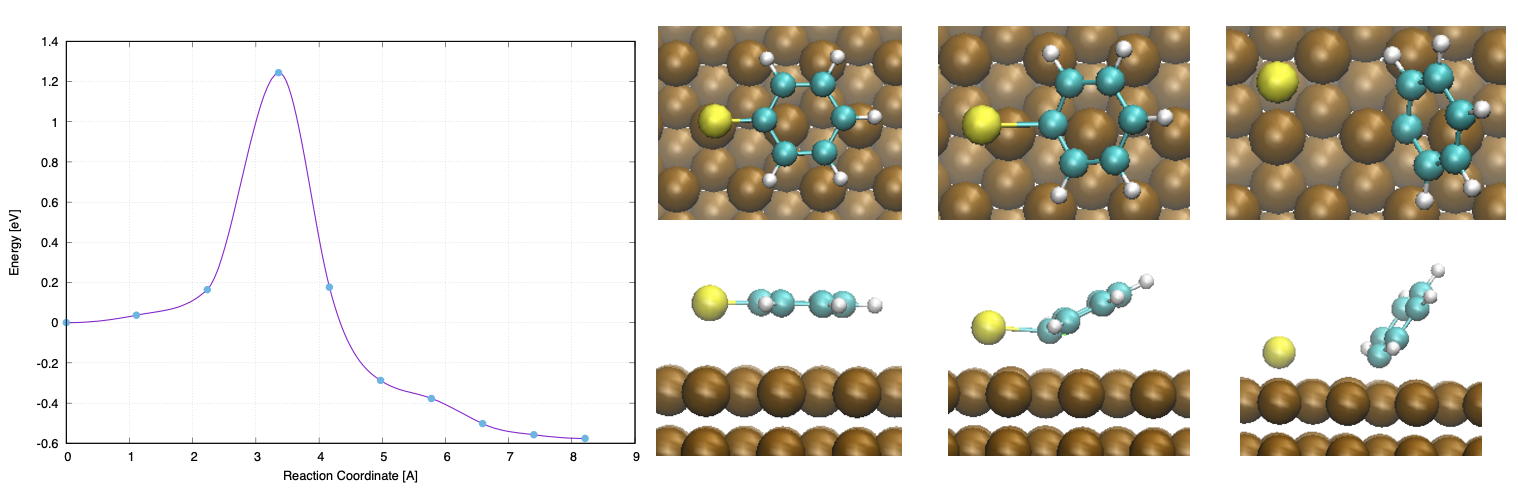
\includegraphics[width=1.0\textwidth]{Fig/dissociation_Cl.png}
\caption{The dissociation of C-Cl bond on Cu(111) surface, left is the energy diagram of the CI-NEB calculations, right side are the top and side view of $IS$, $TS$ and $FS$. (Sphere with ochre color is copper atoms, with cyan color is carbon atoms, with white color is hydrogen atoms. Same in below models. Sphere with yellow color is chlorine atom)}
\label{fig:dissociation_Cl}
\end{figure*}

\begin{figure*}[hbt]
\centering
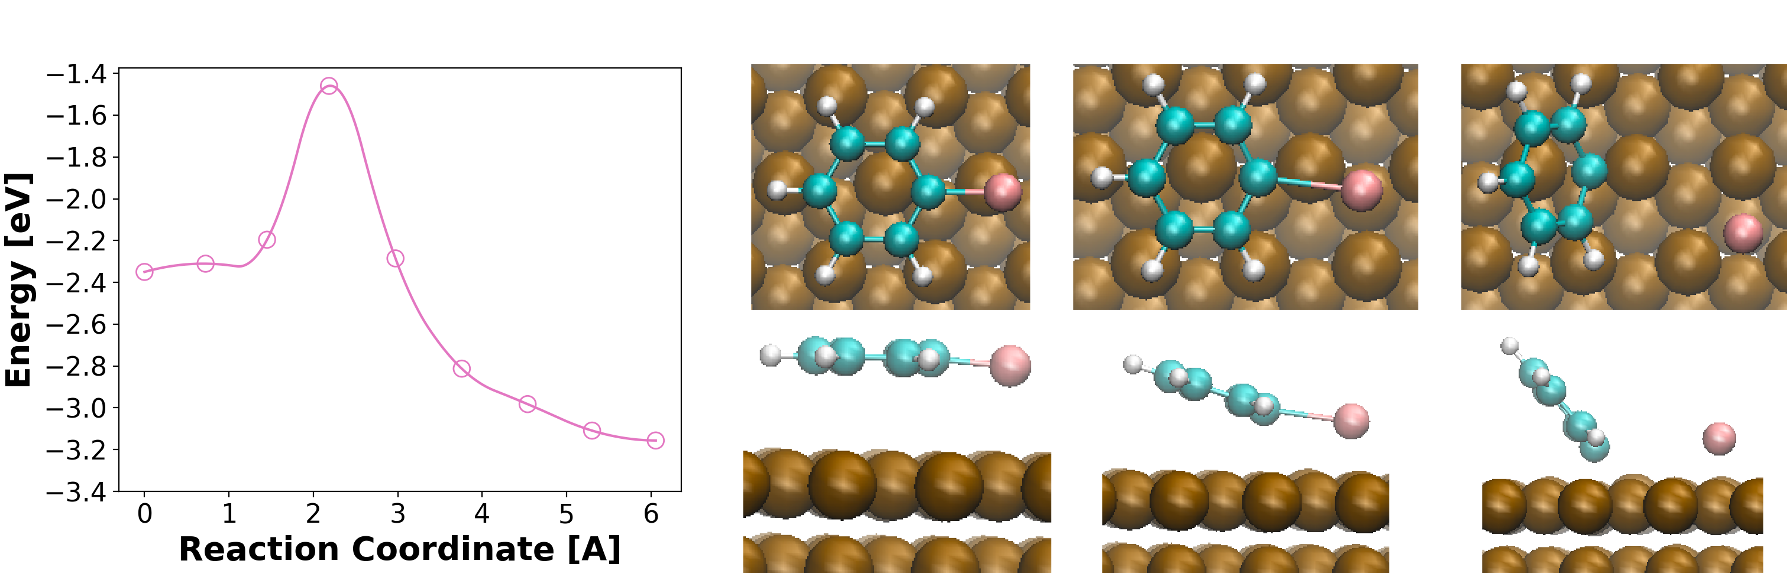
\includegraphics[width=1.0\textwidth]{Fig/dissociation_Br.png}
\caption{The dissociation of C-Br bond on Cu(111) surface. (Sphere with lime color is bromine atoms)}
\label{fig:dissociation_Br}
\end{figure*}

\begin{figure*}[hbt]
\centering
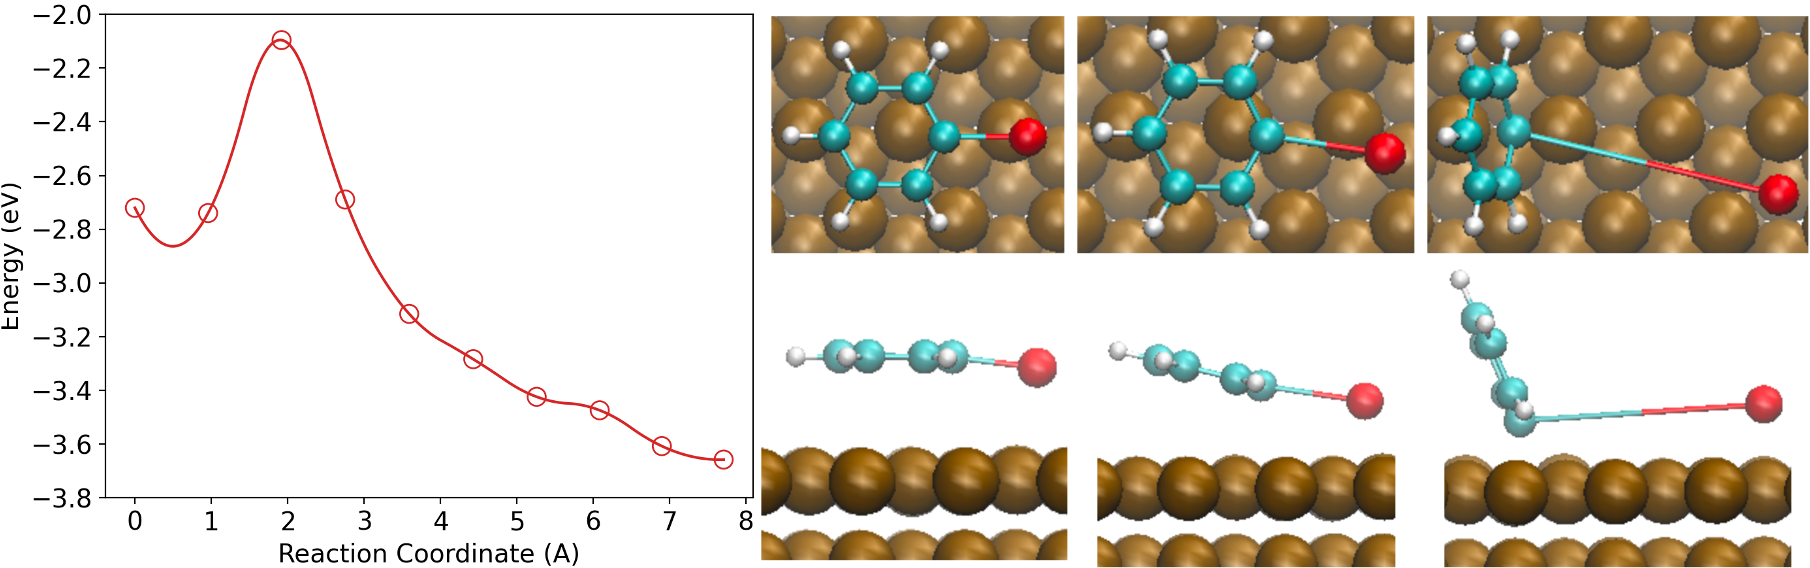
\includegraphics[width=1.0\textwidth]{Fig/dissociation_I.png}
\caption{The dissociation of C-I bond on Cu(111) surface. (Sphere with red color is iodine atoms)}
\label{fig:dissociation_I}
\end{figure*}

\subsection{Diffusion and Formation of Dimerized Organometallic Intermediates}

%R1111: do not use "would". State facts with certainty. "To for a C--C bond the diffusion MUST brings two phenyl groups together."
After the dehalogenation, the diffusion of all species on copper surface would possibly bring two orientation-matched phenyl groups together, leading to the formation of dimerized organometallic intermediates. Since the halogens such as chlorine, bromine and iodine have been dehalogenated and then chemisorbed by the surface, these three different precursors can be fairly considered to form the same dimerized organometallic intermediate structure in this step.

Fig.~\ref{fig:organometallicintermediate} shows the optimized geometry of dimerized organometallic intermediate on Cu(111) surface. From the left picture, it is apparent that these two phenyl groups both conducted interactions with the copper atom on Cu(111) surface; from the right side, it shows that, the copper atom that interacted with two phenyl groups is partially lifted from the first layer flat. This metal atom belongs to $nature(1)$. And this phenomenon does not take place when there is only one phenyl group since the interaction is not strong enough. 

%R1111: Why chlorobenzene is so different? Halogen does not participate in this step at all. How come that the reaction energy is so different?
Besides, the enthalpy of the reaction for three precursors from dehalogenated chlorobenzene, bromobenzene and iodobenzene to dimerized organometallic intermediate are +1.40 eV, +0.17 eV and +0.17 eV, respectively. These three reactions are all endothermic, and the dehalogenated chlorobenzene will adsorb the most energy, which is consistent with the experiment that transformation to dimerized organometallic intermediates from dichlorobenzenes wound not be completed unless a higher temperature is present, but transformation of dibromobenzenes and diiodobenzenes would fulfill at room temperature.

%R1111: It looks like this unfinished paragraph belongs to the next subsection: formation of the C--C bond.
Here, we considered that the dimerized organometallic intermediates were formed with the copper atom of $nature(1)$. In reality, the copper atom in organometallic intermediates may also come from the adatom which is of $nature(2)$. It will lay above the surface before the coupling reaction occurs. In this case -----

%R1111: This intermediate is shown in the figure for the C--C bond formation. Remove this figure, re-reference.
\begin{figure}[hbt]
\centering
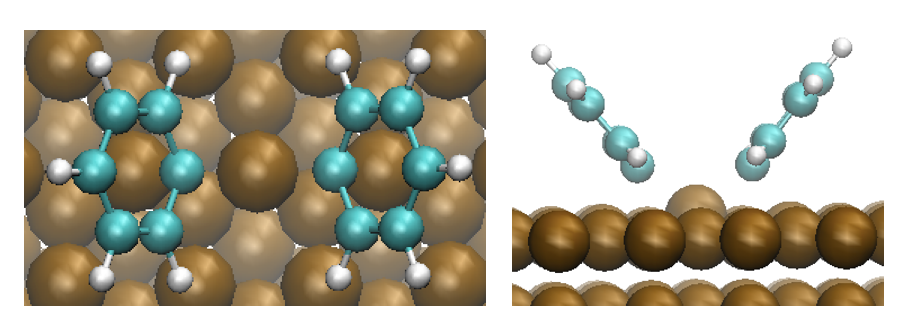
\includegraphics[width=0.45\textwidth]{Fig/organometallicintermediate.png}
\caption{The organometallic intermediate on Cu(111) surface}
\label{fig:organometallicintermediate}
\end{figure}

\subsection{Formation of Carbon Carbon (C--C) Bond}

The final coupling step is the formation of carbon carbon bond (C--C). As discussed above, we explored the two pathways of the C--C bond formation starting from  the Cu atom partially lifted from the surface by two phenyl groups. In the first pathway (Path~1), the Cu atom returns back to its original position in the first surface layer once the C-C bond is formed without producing an adatom. In the secind pathway (Path~2), the Cu atom is pulled out from its original position to become an adatom and leaving the vacancy in its original position. %This means that the metal atom is of $nature(1)$ at the beginning of surface Ullmann coupling, and in the end it changes to $nature(2)$ through the $origin(2)$ method, becoming a new adatom on metal surface.
Here, we investigated two possibilities separately.

\subsubsection{Path I: Cu Returns to Original Location after Coupling Reaction}

%R1111: LATER. We need to develop better notation for all chemical species and refer to them consistently.
%R1111: comparison to existing calculations. Comparison between different metals (and halogens?) in our own calculations.
In Path I, the formation of C--C bond started from the dimerized organometallic intermediate in which the copper atom was partially lifted (notated as $IS_{path1}$). Then the two carbons which would construct a new bond later slope closer to each other, while the copper atom was less lifted on the surface (notated as $TS_{path1}$). Finally, a new C-C bond was formed and the surface went back to original configuration, no adatom forms after the coupling reaction finished (notated as $FS_{path1}$).

In Fig.~\ref{fig:bondformlift}, along the potential energy surface, 6 intermediates were interpolated between $IS_{path1}$ and $FS_{path1}$. The tilt angle of phenyl species in respect to the Cu(111) surface was $50^\circ$ in $IS_{path1}$ and flattened to $35^\circ$ in $TS_{path1}$ and ended at $0^\circ$ in $FS_{path1}$. The distance between the two carbon atoms which would construct a bond varied from 3.10 \AA\ to 2.28 \AA\ and ended at 1.49 \AA\.

Path I reaction is exothermic, the enthalpy $\Delta H$ is -2.00 eV, and $E_{barrier}$ is 0.50 eV.
%R1111: This results agree with the computational study of the C--C formation of dibromobenzene species. Reference.

%R1111: LATER. It is important to discuss the zero-energy for this step. Would it be more informative to use a common zero from the entire energy profile?
\begin{figure*}[hbt]
\centering
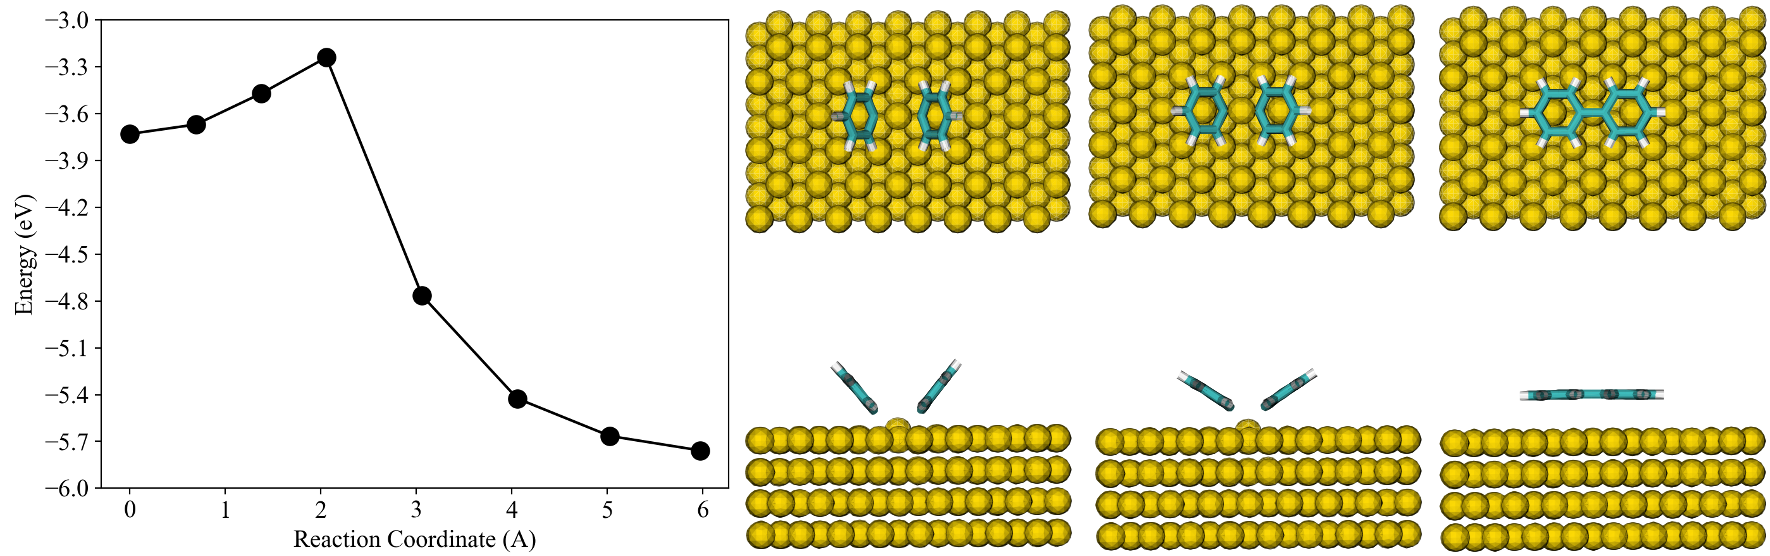
\includegraphics[width=1.0\textwidth]{Fig/bondformlift.png}
\caption{C-C bond formation through lifting Cu atom Path I}
\label{fig:bondformlift}
\end{figure*}


\subsubsection{Path II: Cu becomes a new adatom after coupling reaction}

In Path II, the process started from the organometallic intermediate whereh the copper atom is fully pulled out as an adatom (notated as $IS_{path2}$) (here we created a vacancy on surface corresponding to the creation of adatom, to assure the whole system has the same number of atoms). Then the two phenyl groups would be lifted higher and closer to each other, while the copper atom is less lifted and move towards a hollow site on the surface(notated as $TS_{path2}$). Finally, a new C-C bond is formed and a new adatom and a new vacancy are created on the surface (notated as $FS_{path2}$).

As Fig.~\ref{fig:bondformadatom} show, in this path, 10 intermediates were interpolated between $IS_{path2}$ and $FS_{path2}$.The tilt angle of phenyl species in respect to the Cu(111) surface initialized at $8.5^\circ$ and $12.2^\circ$ in $IS_{path2}$ (the difference angle could be accounted by the fact that vacancy is close the one phenyl species, this will affect a little on the tilt angle), then flattened to nearly $0^\circ$ in $TS_{path2}$ and ended at $-9.1^\circ$ in $FS_{path2}$ (the negative angle arises from the fact that the adatom is right behind the biphenyl). The distance between the two carbons which would construct a bond varied from 3.89 \AA\ to 2.53 \AA\ and ended at 1.50 \AA\ .

Path II reaction is slightly exothermic, the enthalpy $\Delta H$ is -0.17 eV, and $E_{barrier}$ is 2.00 eV, higher than the $E_{barrier}$ of Path I.

\begin{figure*}[hbt]
\centering
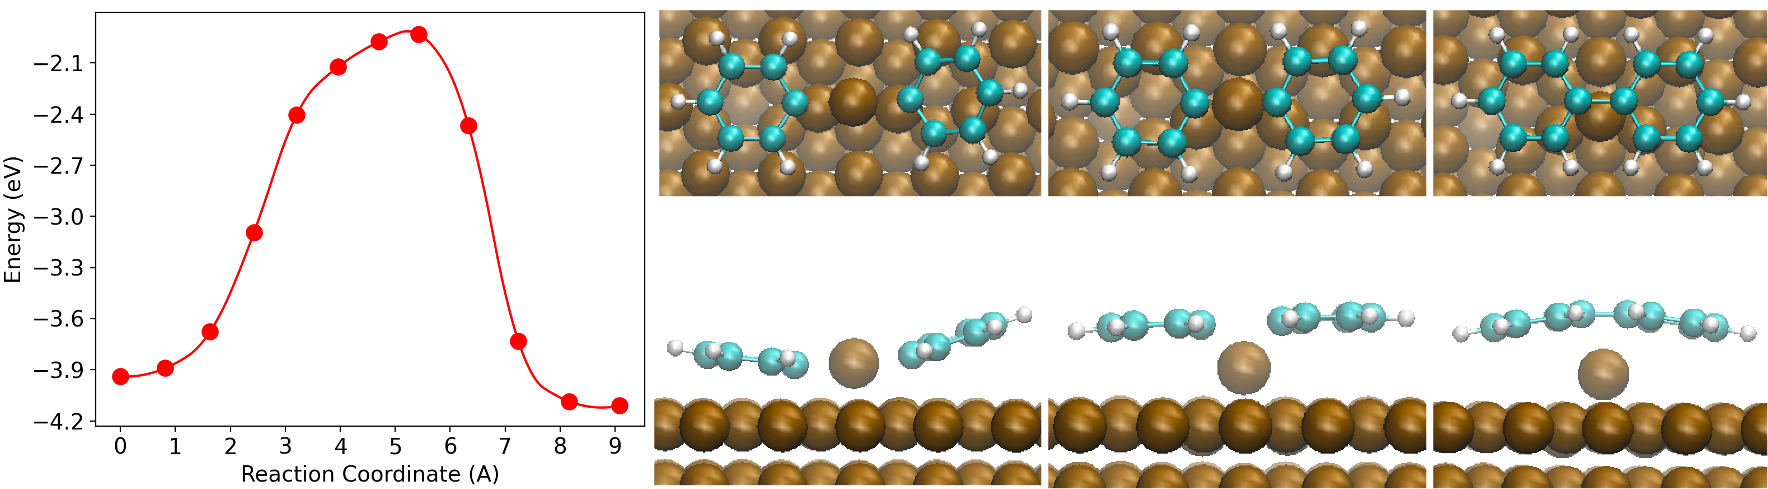
\includegraphics[width=1.0\textwidth]{Fig/bondformadatom.png}
\caption{C-C bond formation through new formed adatom Path II}
\label{fig:bondformadatom}
\end{figure*}

%R1111: All titles and subtitles use sentence case, meaning only the first word is capitalized.
\subsubsection{Path I vs path II}

Taking the data of Path I and Path II into consideration, finally, a feasible C--C bond was constructed in both cases (bond length is around 1.5 \AA\, expected to be 1.34 \AA\ - 1.54 \AA). From thermodynamic aspect, Path I is much more exothermic, which means it will lead to a more stable product. Kinetically, the activation energy of Path I is also smaller than Path II, which means at the same temperature, the Path I reaction would take place at a higher speed and account for a much larger percentage. In this case, we could safely conclude that, if there is no pre-exiting adatom on copper surface, the formation of C--C bond in surface Ullmann coupling will follow the path I.

%R1111: Compare C--C distance in IM4 and IM5 to the experimental data for Ph-Halogen. Can we see IM5 experimentally? 3.89Ang vs 3.1Ang.


%R1111: Note that the difference between dimer1 and dimer2 is smaller than the difference between FS1 and IS. Probably because the dimer interacts stronger with the adatom than with the surface. 


\subsection{Energy diagram of complete Surface Ullmann Coupling Reaction}
In this section, the summary of thermodynamic data of all intermediates in surface Ullmann coupling reaction is present in one diagram. As is shown in Fig.~\ref{fig:completeenergy}.

Here taking the surface Ullmann coupling between two bromobenzene as example, the physisorption of two bromobenzene on Cu(111) surface decrease the energy of the whole system by 2.35 eV, which is widely recognized in experiment because adsorbing aromatic species on copper surface as a fast procedure. 
Then till the formation of new C--C bond, a detailed discussion has been demonstrated in previous sections. The last two successive steps are concerned with the desorption of biphenyl molecule and two dehalogenated bromine atoms. 
In total, the red line is more energetically favourable than green line, that can be considered to be a more reasonable pathway in realistic surface Ullmann coupling if there is no pre-exiting adatom on metal surface.

%%% Early steps
%R1111: LATER. Do we need adatom calculations for TS1? Perhaps only one or two halogen-metal pairs (for complete diagram). How will it affect the subsequent steps? Will the PH-Adatom roam the surface together before encountering the second Ph? PRIORITY6.
%R1111: Why there is no Cu-atom lifting during the C-X bond dissociation? Compare to previous works. Actually partial lifting is a process with a barrier for Au and Ag surfaces but not for Cu. We might need to reproduce this after all. --> More comparison to the existing calculation is required.

%%% Late steps
%R1111: Is the later part of the diagram halogen independent? YES!
%R1111: The barrier between IM4 and IM5 is important. Because it seems that it exists when the adatom is pulled by the R-X dissociation. PRIORITY2. Use NEB to find it.
%R1111: We need free energy for the important IM4->IM5 step. This will include increased entropy of the adatom-vacancy system (assuming that the atom with two phenyls diffuse freely). PRIORITY4.
%R1111: What is the energy of the state after dimer1, when the dimer "falls" flat to the surface? It should be around -3.97 eV. dimer1-2: dimer2+fs1-IS-IS=-3.97 eV
%R1111: An alternative TS2-1 must be calculated. The final product should be lying flat on the surface. PRIORITY3.
%R1111: What effect is responsible for the energy lowering upon adatom creation in IM5? Note that for I--Ph on Cu the extraction+diffusion during the C-I breaking step produces the overall uphill step. PRIORITY1. Remove Ph in IM3, IM4, IM without geometry relaxation (only the metal surface, not phenyl).

%%% Minor comments
%R1111: State labeling is poorly planned. Relabel states to stick to one system.
%R1111: Should we add one more TS between IM2 and IM3? LATER.
%R1111: How does the vacancy affect the energy? LATER.
%R1111: Halogen filling the vacancy or sitting on top of the adatom? PRIORITY5.

\begin{figure*}[hbt]
\centering
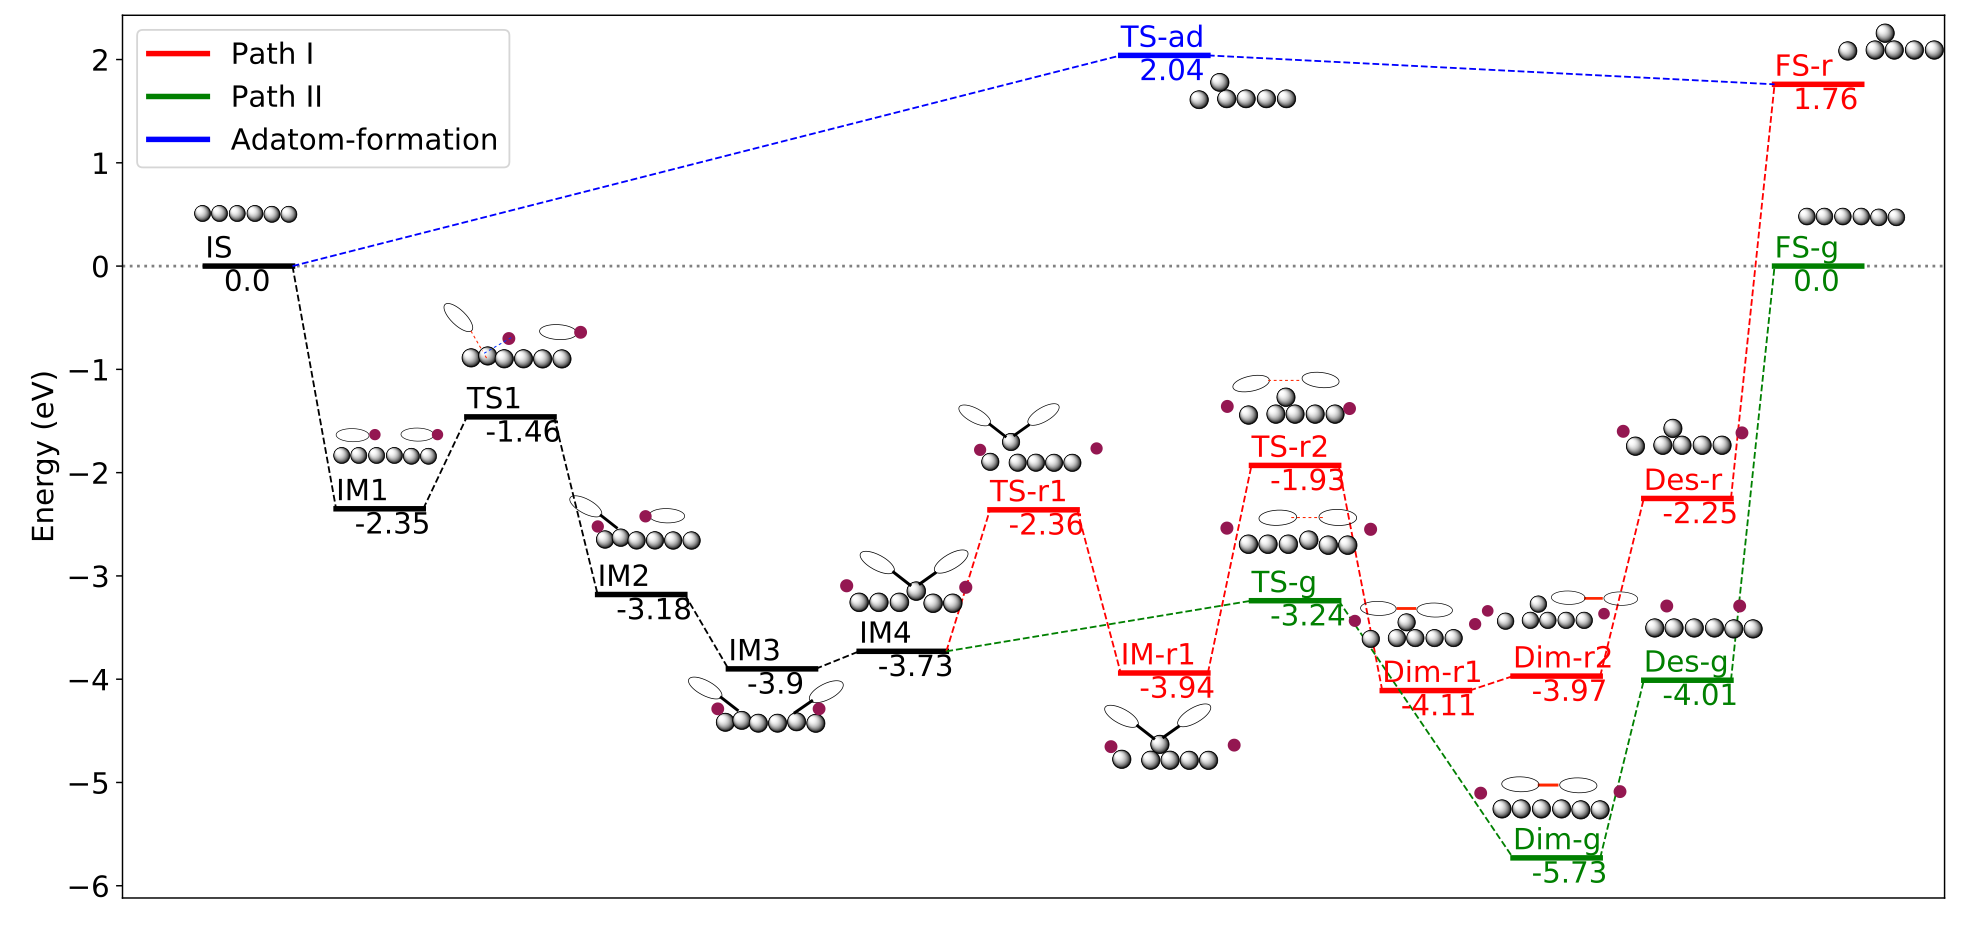
\includegraphics[width=0.98\textwidth]{Fig/completeenergy.png}
\caption{The Energy Diagram of Surface Ullmann Coupling Reaction.
the red line is the surface Ullmann Coupling reaction following Path II, the green line is following Path I. Finally, red line ended with a adatom-vacancy pair on Cu(111) surface and the green line ended same as the original Cu(111) surface.(red circle means bromine atoms)}
\label{fig:completeenergy}
\end{figure*}

\subsection{Formation of Adatom on Pure Cu Surface}

Finally, the energy of forming an adatom on a perfect Cu(111) surface is also presented. The goal of showing this energy diagram is to launch a comparison between two different conditions, both of which deliver an adatom on Cu(111) surface. One is the formation without any species on metal surface, the other one is with surface Ullmann coupling reaction.
As Figure.~\ref{fig:pureadatomform} shows, the reaction of forming a new adatom-vacancy pair on perfect Cu(111) surface is endothermic, $\Delta H$ is 1.76 eV and the $E_{barrier}$ is 2 eV. This means at room temperature, the formation of adatom is unfavourable. 
However, as is shown in Fig.~\ref{fig:completeenergy}, the presence of organometallic intermediate in surface Ullmann coupling could promote the formation of adatoms on surface both thermodynamically and kinetically. This pathway might be considered as a plausible method to create adatoms on metal surface.

\begin{figure*}[hbt]
\centering
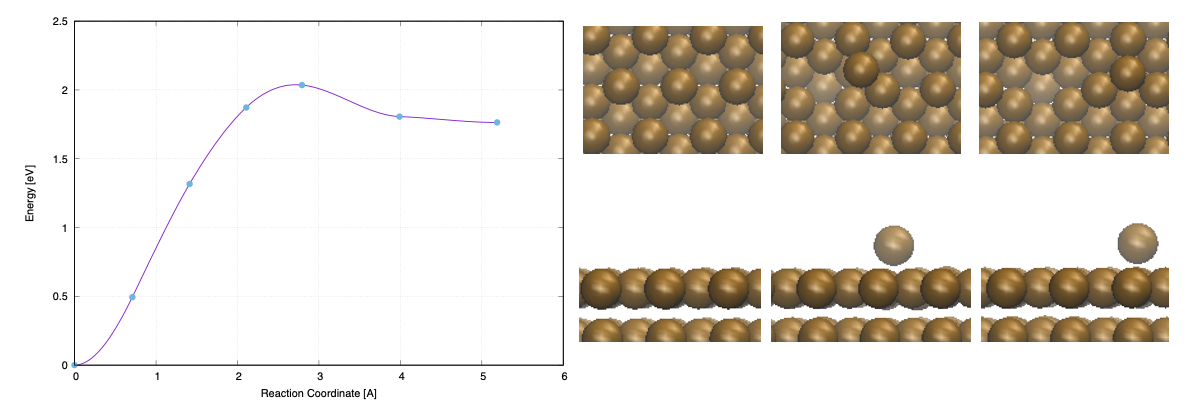
\includegraphics[width=1.0\textwidth]{Fig/pureadatomform.png}
\caption{adatom formation on pure Cu(111) surface}
\label{fig:pureadatomform}
\end{figure*}

\section{conclusions}

\section{acknowledgements}






List of additional reference, not yet encorporated into the manuscript:

\href{https://doi.org/10.1016/j.apsusc.2020.145797}{Ullmann coupling of 2,7-dibromopyrene on Au(1 1 1) assisted by surface adatoms}










\nocite{*}

\bibliographystyle{apsrev4-1} % Tell bibtex which bibliography style to use
\bibliography{references}% Produces the bibliography via BibTeX.

\end{document}
%
% ****** End of file apssamp.tex ******
